%name: Kotha vvsn Tarakesh
%regno:23MIS7039
%Email: tarakeshkotha@gmail.com
%ORCID:0009-0002-2677-4525

\documentclass[a4paper,fleqn]{cas-dc}

\usepackage[numbers]{natbib}
\usepackage{mathtools}
\usepackage{booktabs}
\usepackage{flushend}
\usepackage{graphicx}
\usepackage{algorithm}
\usepackage{algorithmic}
\usepackage{amsmath}
\usepackage{amssymb}
\usepackage{tikz}
\usepackage{subcaption}
\usepackage{float}
\usepackage{placeins}
\usepackage{needspace}
\usepackage{pgfplots}
\usepackage{tikz}
\usepackage{xcolor}
\pgfplotsset{compat=1.17}

\definecolor{myblue}{RGB}{54,106,146}
\definecolor{mygray}{RGB}{240,240,240}


\numberwithin{equation}{section}

\begin{document}
\let\WriteBookmarks\relax
\def\floatpagepagefraction{1}
\def\textpagefraction{.001}

\shorttitle{Cross-Layer Security-Performance Trade-Off Analysis in Wireless IoT Networks}
\shortauthors{Kotha VVSN Tarakesh et~al.}

\title [mode = title]{Cross-Layer Security-Performance Trade-Off Analysis in Wireless IoT Networks}

\author[1]{Kotha VVSN Tarakesh}[orcid=0009-0002-2677-4525]
\ead{satya.23mis7039@vitapstudent.ac.in}
\address[1]{School of Computer Science and Engineering, VIT-AP University, Amaravathi, Andhra Pradesh, India}



\begin{abstract}
There are many billions of devices  connected wirelessly throughout the Internet of Things (IoT) in various sectors such as healthcare services, smart cities, automotive and transportation, and industrial systems. The ability to connect these devices wirelessly allows for efficient data sharing; however, this interconnectedness has also exposed IoT infrastructures to numerous types of cyber attacks. Traditional network security measures tend to perform poorly in IoT environments due to the limited power supply, limited processing capabilities, and highly dynamic nature of most wireless IoT networks that are created as a result of their various use cases. Additionally, the characteristics associated with a high volume of data and traffic in IoT networks make it difficult for reliable intrusion detection to be performed on these networks. This research intends to examine the relationship between security measures and communication performance in wireless IoT networks, specifically investigating how implementing cross-layer security design can provide enhanced security assurance with a manageable resource usage.
\end{abstract}

\begin{keywords}
Internet of Things (IoT) \sep
Cross-Layer Security \sep
Intrusion Detection System (IDS) \sep
Machine Learning \sep
Energy Efficiency \sep
Adaptive Secure Routing \sep
Security-Performance Trade-Off \sep
Wireless IoT Networks
\end{keywords}

\maketitle

\section{Introduction}

As a result of the rapid growth of IoT, billions of connected devices have been deployed in a variety of sectors, including healthcare, smart cities, industrial automation, and transportation systems. These devices continuously share sensitive data over wireless channels and therefore have a high exposure to cyber attacks and privacy breaches.\cite{etman2025mlwsn}.Unlike traditional computing systems, IoT nodes are generally limited in their processing capability, memory capability and energy capability so deploying traditional security mechanisms are problematic. Therefore, IoT networks require lightweight, adaptive, and dynamic wireless security solutions

Studies (surveys) have shown that effective IoT security cannot be achieved through the isolated deployment of protective mechanisms at a specific protocol layer.\cite{kaur2024ris}.Studies (suThere are several physical-layer security approaches including but not limited to cooperative jamming and reconfigurable intelligent surfaces that can promote confidentiality as well as resiliency against eavesdropping\cite{martalo2024crosslayer}. However, each of these approaches impose additional overhead with respect to energy and signaling, thereby degrading communication performance in resource constraint IoT environments.For example, attacks that are directed at either the physical or MAC layers can move up to the upper layers causing harm to both data integrity and application services. 

Due to their ability to identify intricate and evolving threats through analysis of network traffic data, machine learning has become an important tool for enhancing the security of IoT systems \cite{mustafa2025ml}.Machine-learning-based IDS have the capability of adapting to new threats more successfully than rule-based IDS and are therefore well-suited for use in dynamically changing IoT networks. However, while machine-learning models require both computational and communications resources to train and run, inadequate optimization may result in a decrease in overall system performance. Therefore, balancing security and operational efficiency remains an important issue.

Several recent studies have emphasized the need for the development of cross-layer security designs that coordinate security functions across the physical layer, networking layer, and application layer \cite{cetintav2025auth}. Cross-layer solutions may achieve greater efficiency by exchanging information between layers, which allows for a reduction in redundant processing. However, current cross-layer frameworks tend to focus on improving security or optimising performance as separate problems and do not usually attempt to simultaneously pursue both objectives. As a result, most cross-layer frameworks are not practical for large-scale deployments of wireless IoT systems where all three of the following attributes are desired: energy efficient, low-latency, and secure.

This research paper provides an overview of the study of how to make sure that the Wireless Token and the Value Ad Network (IoT, or intelligent things that use a wireless connection to send and receive data) operate securely and efficiently. Specifically, this study compares the tradeoff between security and performance attributes in an IoT.

\subsection{Contribution of this work}

The paper takes a holistic view on IoT security by telling you what IoT security currently exists. Specifically, the paper addresses the three levels of IoT security: the MAC layer, network layer, and application layer. One of the unique aspects of this study is that it does not look at these three levels of IoT security in isolation; rather, it demonstrates that decisions made about IoT security policies at one level may impact both the power required to use the IoT node and the amount of time an IoT node takes to complete a process at the three levels of IoT security.

This research focuses on integrating physical-layer security, intrusion detection using machine learning, and lightweight authentication. It studies the integration of these technologies in order to better achieve confidentiality, integrity, and availability of communications while minimizing the resource usage by IoT devices.

The research highlights the interrelatedness of these technologies by providing an organization system and a comprehensive summary chart of various technologies. This will be useful for both researchers who study them and for potential users of the research, as they will be able to evaluate different technological implementations in terms of the level of security provided during communication as well as the level of energy consumed in different IoT "use cases." This research also describes how to balance security, efficiency, and energy usage, in IoT use cases, based on the various potential use cases of IoT.

Research indicates that there are serious deficiencies in today's cybersecurity solutions. For example, current security technologies lack adaptability when required (i.e., in response to changing network conditions), and security policies are poorly aligned with machine learning-based optimizations. The research presents examples of these deficiencies based on a new multi-layered approach to securing networks.


In summary, the results of the research provide a strong rationale for developing future cross-layer security/performance optimization frameworks that will allow for scalable, energy-efficient, and resilient wireless IoT systems.




\subsection{Organization of the Article}

This document is arranged into several sections. Section two highlights the concept of cross-layer security; describing the relationship between security and performance across the attributes of Wireless IoT Networks.

Section three references literature that is related to this area of interest; examining security mechanism implementations, such as physical layer security and machine learning based methods to discover intruders as well as mechanisms to improve the ease of performing authentication and methods to optimize the cross-layer security experience. This section also highlights deficiencies found in both the current cross-layer security mechanisms and other areas of wireless IoT networks. Section four provides a more detailed examination of the security versus performance tradeoff relationship and examines how these security mechanism affect Energy, Latency and Reliability. Finally, section five summarizes the document and provides information on future research opportunities in optimizing security and performance across the layers of wireless IoT systems.

\section{Research Objectives}



In this research we will study the types of security measures implemented in the Internet of Things networks and their impact on the energy used, the amount of time to transmit and the cost of communicating at the different levels. We will also determine how the security measures of how encryption, authentication, and/or intrusion detection can be used to improve how the Internet of Things devices operate.



We will then examine different research conducted on security frameworks across different levels, and explore how these levels work together to affect how effectively internet of things devices communicate with one another. Our goal in this research will be to determine if providing a means of sharing information across these levels increases the overall security and efficiency of Internet of Things devices in comparison to if each level were to operate independently.



Lastly we will explore using technologies that could include machine learning, lightweight encryption techniques and automated intrusion detection systems to achieve a balanced security for Internet of Things devices. We will focus on how changeable and adaptable models can reduce the amount of processing and energy required while still protecting Internet of Things networks from ever changing threats.

The ultimate goal is to establish the key gaps limitations in the current cross‐layer security frameworks and to develop a framework developed from those findings that can support cross‐layer security performance‐trading in future IoT system design.



\subsection{Additional Objectives}

In addition, this research project has several secondary objectives which will help provide more in‐depth understanding that exists regarding the security-performance trade‐offs in the field of IoT networks. First, this report will perform an objective comparative analysis of the various categories of security mechanisms (i.e., physical layer security, cryptographic algorithms, machine-learning based intrusion detection, etc.) based on their respective impacts upon energy consumption, latency and communication overhead. This comparative analysis will help to determine which of the security techniques would be best suited for use in resource-constrained IoT devices.



Second, this work will look at how sharing cross-layer information can help to coordinate the actions taken by different layers of protocol. Exchanging security-related information and performance data between the physical, MAC, network, and application protocol layers will allow IoT systems to eliminate redundant operations, thus enabling more effective resource allocation, improved routing, and enhanced enforcement of security policies.

This study also seeks to evaluate the influence of different IoT deployment scenarios, such as smart cities, healthcare systems, industrial automation, and environmental monitoring, on the effectiveness of cross-layer security approaches. Since each of these environments has distinct traffic patterns, reliability requirements, and energy constraints, understanding their impact on security design is an important goal of this work.

Another objective is to investigate how emerging technologies, such as edge computing, artificial intelligence, and intelligent wireless surfaces, can support more efficient and secure IoT communications. By integrating these technologies into cross-layer security frameworks, it becomes possible to improve both the responsiveness and robustness of IoT systems.

The paper also aims to analyze the trade-offs between centralized and distributed security architectures. While centralized approaches may offer better control and global visibility, distributed security mechanisms are often more scalable and resilient in large and heterogeneous IoT networks. Understanding these trade-offs is essential for designing practical and scalable security solutions.

Furthermore, this work seeks to study how adaptive and context-aware security mechanisms can respond to changes in network conditions, traffic loads, device mobility, and attack patterns. Adaptive security is particularly important in wireless IoT environments, where network conditions and threats can change rapidly.

Another important objective is to assess how learning-based optimization techniques, such as reinforcement learning and deep learning, can be integrated with security policies to achieve a better balance between protection strength and system performance. This includes evaluating how these techniques can reduce unnecessary security overhead while maintaining high levels of protection.

Finally, this study aims to provide practical design guidelines for researchers and system developers. These guidelines will help in selecting and configuring cross-layer security mechanisms based on the specific energy, latency, and reliability requirements of different IoT applications. By addressing both theoretical and practical aspects, this work contributes to the development of more secure, efficient, and scalable wireless IoT systems.


\section{Cross-Layer}

\subsection{Cross-Layer Security Architecture for IoT}

Research has shown that single‐layer security solutions are not sufficient for protecting wireless IoT networks, which are exposed to different types of attacks at various layers of communication. Cross‐layer security architectures combine protection mechanisms at the physical, network, and application layers to provide more comprehensive defense. The approach described in \cite{musaddiq2020rl} demonstrates that using machine learning based anomaly detection at the MAC layer together with adaptive encryption at the application layer improves both security and energy efficiency. Similarly, the survey in \cite{kaur2024ris2} reports that cross‐layer coordination can reduce latency and security overhead, leading to more reliable IoT communications.

\subsubsection{Physical Layer Security}

Physical layer security focuses on improving confidentiality by using the characteristics of wireless channels instead of relying only on cryptographic methods. Techniques such as cooperative jamming and reinforcement learning based power control can increase secrecy capacity by managing interference \cite{martalo2024crosslayer2}. Reconfigurable intelligent surfaces further enhance legitimate communication while making eavesdropping more difficult \cite{kikissagbe2024ids}. Although these methods are effective, they also introduce additional computation and energy usage, which must be carefully managed in IoT environments where resources are limited.

\subsection{Machine Learning and Performance-Aware Security in IoT}

Machine learning has become an important tool for IoT security because it can detect complex and changing attack patterns in network traffic. The cross‐layer framework presented in \cite{altalhan2025imbalance} shows that lightweight learning models operating across multiple layers can achieve high detection accuracy without excessive computational cost. In addition, the study in \cite{etman2025mlwsn2} highlights that machine learning can improve data integrity and resource utilization in wireless sensor networks. At the same time, learning‐based security methods increase processing and communication overhead, which makes it necessary to design security mechanisms that are aware of their impact on performance.

\subsection{Recent Advances in IoT Security}

Recent work in IoT security emphasizes the use of intelligent and adaptive mechanisms to deal with increasingly complex cyber attacks. Traditional rule‐based systems are often unable to cope with the dynamic nature of IoT networks, which has encouraged the adoption of machine learning and deep learning based intrusion detection systems. These techniques are capable of identifying both known and previously unseen attacks with relatively high accuracy.

Recent surveys also point out the importance of deploying security measures across multiple layers of the communication stack rather than relying on a single defense point. Combining application‐level authentication, network‐level anomaly detection, and physical‐layer protection improves the overall resilience of IoT systems. However, this integrated approach also increases energy consumption and communication delay, reinforcing the need to carefully study security–performance trade‐offs in wireless IoT networks.
\begin{table*}[htbp]
\centering
\caption{Summary of Recent Studies on Cross-Layer Security and Performance Trade-Offs in Wireless IoT Networks}
\label{tab:literature}
\renewcommand{\arraystretch}{1.15}
\setlength{\tabcolsep}{6pt}
\footnotesize

\begin{tabular}{|c|p{3.2cm}|p{4.0cm}|p{4.0cm}|p{4.0cm}|}
\hline
\textbf{Ref} & \textbf{Focus Area} & \textbf{Methodology} & \textbf{Key Contributions} & \textbf{Limitations} \\
\hline

\cite{etman2025mlwsn} & Cross-layer intrusion detection and encryption & Machine learning based anomaly detection and adaptive encryption & Improved attack detection and reduced energy consumption & Model training introduces computational overhead \\
\hline

\cite{kaur2024ris} & Physical layer secrecy optimization & Cooperative jamming and reinforcement learning & Increased secrecy capacity under interference & Additional signaling and power control overhead \\
\hline

\cite{martalo2024crosslayer} & RIS-based physical layer security & Intelligent surface assisted channel control & Enhanced confidentiality and link quality & Deployment complexity and hardware cost \\
\hline

\cite{mustafa2024framework} & Cross-layer IoT security architecture & Multi-layer coordination and adaptive security control & Reduced latency and communication overhead & System complexity increases with scale \\
\hline

\cite{mustafa2025ml} & Machine learning based WSN security & Data analytics and traffic classification & Improved data reliability and resource usage & High training and communication cost \\
\hline

\cite{cetintav2025auth} & Lightweight IoT authentication survey & Cross-layer security analysis, AI-based IDS, and energy-aware networking & Identifies security–energy trade-offs across IoT layers & Survey based and lacks experimental validation \\
\hline

\cite{musaddiq2020rl} & Reinforcement learning based cross-layer optimization & Q-learning, MAC–routing interaction, adaptive parent selection & Reduced energy consumption and improved packet delivery & Training convergence and model stability \\
\hline

\cite{liu2024auth} & Lightweight cross-layer authentication & Channel fingerprinting and energy-aware routing & Reduced authentication overhead and energy use & Sensitive to channel variations \\
\hline

\cite{mohaghegh2024auth} & Survey on cross-layer authentication methods & Channel-based and cryptographic authentication & Identified low-cost authentication solutions & Lack of practical deployment models \\
\hline

\cite{meng2024phyml} & Review of physical and cross-layer authentication & Statistical analysis and machine learning & Comparative evaluation of authentication schemes & Limited focus on performance trade-offs \\
\hline

\cite{mustafa2025phylauth} & Machine learning based physical layer authentication & Signal feature extraction and classification & Reduced cryptographic computation cost & Accuracy depends on channel stability \\
\hline

\cite{mustafa2024energy} & Cross-layer energy consumption modeling & Joint resource and protocol optimization & Reduced overall energy usage & Security aspects not deeply analyzed \\
\hline

\cite{khalil2024connectivity} & Cross-layer connectivity and performance optimization & Adaptive routing and resource allocation & Improved throughput and reduced delay & Security not included in optimization \\
\hline

\end{tabular}
\end{table*}


\section{Literature Survey}

People who study Internet of Things security are saying that the old ways of keeping things secure do not work for Internet of Things. This is because Internet of Things has a lot of devices that do not have a lot of power or ability to do complicated things.

Internet of Things devices have to be careful with energy. They cannot do a lot of complicated calculations. So the big and complicated security methods that need a lot of power are not good for Internet of Things. Some people did studies, like the ones in B4 and B6. They found out that Internet of Things has problems with security, in many areas. This means that we need to find ways to protect Internet of Things at different levels.
People are paying attention to layer security because it is a good way to keep things private without using only secret codes. Studies, in some papers show that working together to block signals and using surfaces that can change how they work can really help keep secrets safe by using the way wireless signals travel. These methods make it very hard for someone to spy on us. They also need more signals and energy to work properly. Physical layer security is still an option because it helps with privacy.

The use of techniques like learning has made physical-layer security even stronger. Some studies, such, as the ones done in \cite{zhang2025dlids} show that reinforcement learning and adaptive power control can really help improve communication when the channel and interference conditions are changing. This means that Internet of Things systems can change their transmission strategies away to keep things confidential. Internet of Things systems can do this because these methods let them adjust in time.

Internet of Things networks are using machine learning to detect intruders. This is a common security measure now. Some people wrote about this in a paper \cite{mustafa2025ml2}. Someone else did a survey \cite{mustafa2025securearch}. They found out that simple machine learning models can find attacks and weird traffic accurately.. The good thing is that these models work well even on devices that do not have a lot of power. Machine learning is used for this because it is good at finding intruders. However training these machine learning models and sharing data still takes up some resources. Machine learning models need to be trained and data needs to be exchanged which can be a problem, for Internet of Things devices.

There have been studies that look at the problems of security that uses learning in Internet of Things. Some research like the kind found in R3 and R4 shows that when the data is not balanced and the ways that people attack are always changing it can make it harder to detect these attacks. This means we need to have learning models that can adapt and be strong. We have to fix these problems if we want to use Internet of Things in life.

Internet of Things security is also using learning and hybrid learning models. Some studies like the ones in \cite{liu2024auth} show that deep learning is really good when it is used with -layer data. This helps to find intrusions accurately and makes the system more reliable.. Internet of Things security models like these need to be optimized carefully so that they do not use too much energy. Deep learning models, for Internet of Things security need to be optimized.

Cross-layer security architectures are meant to keep Cross-layer security architectures across many different protocol layers. Some people did a survey that's in \cite{sreevidya2024trust} and they made a framework to optimize things that is in \cite{khair2024crosslayer}. They found out that when you share information between the layers it helps get rid of stuff and makes Cross-layer security architectures and performance better. This is really helpful in Internet of Things networks, with lots of devices.

People have made some ways to keep things safe when information is being sent between different layers. These new methods are not too complicated. They help keep everything secure. Some researchers found out that using marks to identify channels and choosing routes that use less energy can help reduce the work needed to make sure everything is authentic. This is shown in the work of R9 and R21. They figured out that these methods can help keep the information safe without making things too slow. The goal is to make sure the information that is being sent is real and not fake and that it gets to where it needs to go without any problems.

Other ways to check people are who they say they are across layers can make things more efficient. Some studies like the ones done in \cite{xiao2024multipath} found that using things about the channel and machine learning to check people are who they say they are can really cut down on the need for complicated cryptography, in Internet of Things devices. This means Internet of Things devices do not have to do much heavy work to make sure everyone is who they say they are.

People have been looking at layer and cross layer authentication in recent studies. Some research like the ones, in \cite{martalo2024crosslayer3} show that taking apart signal features and using learning can make authentication more reliable. However the accuracy of layer and cross layer authentication is affected by how much the channel changes.

When we think about Internet of Things security systems we have to consider energy and performance modeling. This is really important for evaluating these systems. Some studies, like the ones in R17 and R29 show that optimizing resources across layers can make a big difference, in how much energy is used and how well the system performs. However the problem is that security is not always a part of these models. We need to make sure that Internet of Things security systems are energy efficient and perform well and that means we have to think about Internet of Things security systems and how to make them better.

Routing and communication efficiency are really important for the Internet of Things to be secure. Some studies, like the ones in R10 and R12 found that using trust and multiple paths to route data can make it more secure. At the time it does not hurt how well the Internet of Things can communicate. The Internet of Things needs to be able to communicate and route data, in a good way to be secure and work properly.

Many people have tried to make protocols and communication. Some studies like the ones in R19 and R24 found out that making the Internet of Things and the edge and the cloud work together smoothly and improving the protocols that applications use can really make things more efficient and reduce waiting time. The Internet of Things and the edge and the cloud are important because they can really affect how well things work. The protocols that applications use are also very important, for the Internet of Things and the edge and the cloud.

When we talk about the Internet of Things, protocol-level optimization is something that really matters for performance. Some studies, like the ones in R26 and R20 show that choosing the protocol and setting it up correctly can make a big difference, in how secure and energy efficient our Internet of Things systems are, especially when we are dealing with a lot of devices.

People who study Internet of Things security have done some surveys. These surveys give us a picture of the Internet of Things security challenges. Some studies, like the ones, in \cite{hu2024physec} tell us about the ways to authenticate Internet of Things and keep the protocols and software safe. They show that we need solutions that work together and can adapt to problems. The Internet of Things security is an issue and we need to find better ways to deal with it.

Overall, the existing literature demonstrates that while a wide range of security and optimization techniques have been proposed \cite{samson2024survey}, most current solutions treat security and performance separately. This gap motivates the need for integrated cross-layer security–performance frameworks that can dynamically balance protection, energy efficiency, and communication reliability in real-world wireless IoT networks.


\subsection{Research Gaps}

Although existing studies provide valuable insights into IoT security, several limitations remain. Most cross-layer approaches focus either on improving security or on optimizing performance, but rarely consider both aspects simultaneously. Physical layer security techniques enhance confidentiality but increase processing and signaling overhead. Similarly, machine learning based intrusion detection improves attack detection accuracy but introduces computational and communication costs. Moreover, existing models often assume static network conditions and do not adapt well to the dynamic and heterogeneous nature of real-world IoT environments.



\subsection{Motivation}

The above limitations highlight the need for security mechanisms that can adapt to changing network conditions while preserving energy efficiency and low latency. Wireless IoT networks require protection frameworks that are not only strong against attacks but also lightweight and performance-aware. By jointly considering security and performance across multiple protocol layers, it becomes possible to design systems that achieve better trade-offs between protection strength and operational efficiency.

\subsection{Problem Statement}

Despite significant progress in IoT security research, there is still a lack of integrated frameworks that jointly optimize security, energy consumption, and communication performance in wireless IoT networks. Existing solutions either focus on isolated layers or introduce excessive overhead that degrades system efficiency. Therefore, there is a need to develop a cross-layer security–performance trade-off framework that can provide strong protection while maintaining acceptable energy usage, latency, and reliability in resource-constrained IoT environments.

\section{Proposed Cross-Layer Security Framework}

\subsection{Overview of the Proposed Framework}

The suggested framework presents a security/performance optimising architecture at different layers for wireless IoT networks, focusing on the balance between protection and communication efficiency in resource-constrained environments. Rather than treating security mechanisms within each layer purely as stand-alone components of the communication stack, the proposed architecture allows for information sharing between the various layers (e.g., the Physical Layer, MAC Layer, Network Layer).

In the proposed architecture, lightweight security mechanisms integrated with adaptive network control mechanisms will dynamically change the level of protection depending on the current state of the networks. Physical Layer security methods provide protection against eavesdropping by using information about characteristics of the wireless channel; MAC Layer lightweight authentication and anomaly detection methods allow monitoring of communication behaviour and detecting possible attacks; and adaptive routing methods at the Network Layer will assist in ensuring reliable delivery of packets while minimising communication overhead.


Machine learning-based Intrusion Detection Systems (IDS) are used to detect anomalous network traffic patterns in the Framework. The Framework can use IDS to identify new attacks at a low cost (in terms of processing resources). The combination of the aforementioned three mechanisms provides for the security characteristics of the Framework, while also providing for the energy conservation aspect of the Framework.
As shown in Figure~\ref{fig:architecture}, the proposed framework coordinates security mechanisms across multiple layers to improve communication reliability and energy efficiency.

The performance of the suggested framework will be assessed through the use of the ns-3 network simulator for network simulations. In this case, many IoT nodes (through wireless links) will communicate with a central sink node while various security mechanisms will be activated. In order to analyse the trade-off between security and communication performance, performance measures such as Throughput, Packet Delivery Ratio, Latency and Energy Consumption will be examined.

\begin{figure*}[t]
\centering
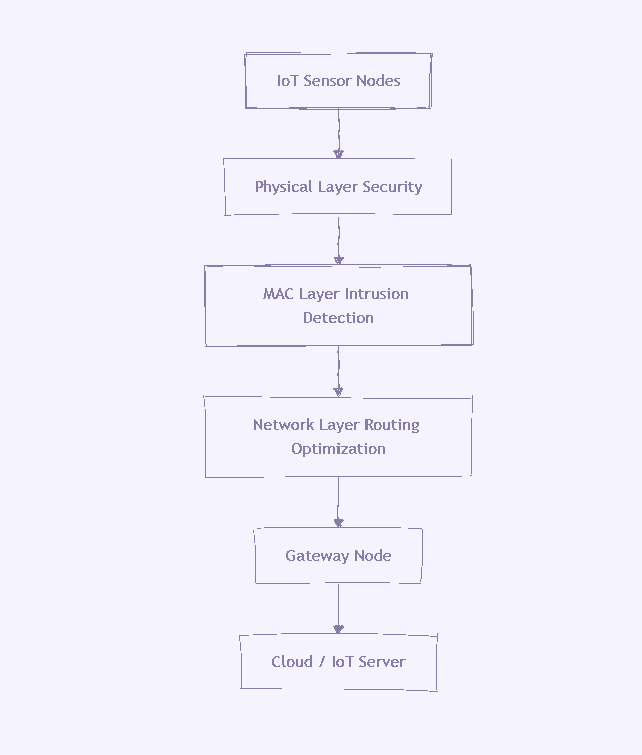
\includegraphics[width=0.6\textwidth]{figures/crosslayer_architecture.png}
\caption{Proposed Cross-Layer Security Framework for Wireless IoT Networks. The architecture integrates physical layer protection, MAC layer intrusion detection, and secure routing mechanisms.}
\label{fig:architecture}
\end{figure*}

\subsection{System Model}

The IoT Network being examined in this research paper consist of an assortment of sensor nodes that are placed throughout an observation area as well as one central location where all data collected from the sensor nodes are sent in the form of data packets over the air via wireless connection from each sensor node.

Assume the wireless network is arranged or structured using N sensor nodes so that each Sensor Node can be designated as:

Let the network consist of N sensor nodes represented as

\begin{equation}
N = \{n_1, n_2, n_3, ..., n_k\}
\label{eq:nodes}
\end{equation}

where \( n_i \) represents the i-th sensor node.

The total energy consumption of a node during communication can be represented as

\begin{equation}
E_{total} = E_{tx} + E_{rx} + E_{proc}
\label{eq:energy}
\end{equation}

where \(E_{tx}\) represents transmission energy, \(E_{rx}\) represents reception energy, and \(E_{proc}\) represents computational energy required for security processing.

The packet delivery ratio of the network is calculated as

\begin{equation}
PDR = \frac{P_{received}}{P_{sent}}
\label{eq:pdr}
\end{equation}

where \(P_{received}\) is the number of successfully received packets and \(P_{sent}\) is the number of transmitted packets.

The throughput of the system is defined as

\begin{equation}
Throughput = \frac{Total\ received\ bits}{Simulation\ time}
\label{eq:throughput}
\end{equation}

These equations allow evaluation of the security-performance trade-off in the proposed framework.

\subsection{Phase 1: Lightweight Authentication Procedure}

In phase one of the proposed design, the intent is to implement simple means of authentication so that only recognized IoT devices may take part in any sort of communication over the network. Because IoT devices typically have limited resource capability, the authentication system must be computationally efficient while at the same time providing very strong levels of security.

Each device will start off sending an authentication request to the gateway. The gateway will evaluate the credentials for that device using lightweight cryptographic functions and generate a session key that will allow the two devices to establish a secure method of communication. The entire process has been designed to minimize latency and energy consumption while preventing unauthorized devices from gaining access to the network.

Finally, the authentication service will adjust the parameters used by the authentication service automatically as the network conditions change, allowing for more adaptive security measures. This also allows for a level of redundancy against replay offenses, impersonation offenses, and unauthorized device entry into the network.

\begin{algorithm}
\caption{Lightweight Authentication Algorithm}
\begin{algorithmic}[1]
\STATE Initialize IoT nodes $N = \{n_1, n_2, ..., n_k\}$
\STATE Initialize authentication database
\FOR{each node $n_i$}
    \STATE Generate authentication request $Req_i$
    \STATE Send request to gateway
    \STATE Gateway receives $Req_i$
    \STATE Extract node ID and timestamp
    \STATE Validate credentials
    \IF{credentials valid}
        \STATE Generate session key $K_i$
        \STATE Encrypt key using lightweight crypto
        \STATE Store key securely
        \STATE Send authentication response
        \STATE Establish secure communication
        \STATE Update authentication log
    \ELSE
        \STATE Reject node request
        \STATE Log unauthorized attempt
    \ENDIF
    \STATE Measure authentication delay
    \STATE Compute energy consumption
\ENDFOR
\STATE Update authentication policy dynamically
\STATE Continue secure network operation
\end{algorithmic}
\end{algorithm}

\textbf{Mathematical Modeling:}

\begin{equation}
T_{auth} = T_{req} + T_{verify} + T_{response}
\label{eq:auth_time}
\end{equation}

\begin{equation}
E_{auth} = E_{tx} + E_{rx} + E_{comp}
\label{eq:auth_energy}
\end{equation}

\begin{equation}
P_{success} = \frac{N_{valid}}{N_{total}}
\label{eq:success_prob}
\end{equation}

\begin{equation}
P_{fail} = 1 - P_{success}
\label{eq:fail_prob}
\end{equation}

\begin{equation}
K_{gen} = f(ID,T,R)
\label{eq:key}
\end{equation}

\begin{equation}
D_{auth} = T_{end} - T_{start}
\label{eq:delay_auth}
\end{equation}

\begin{equation}
C_{auth} = \alpha E_{auth} + \beta T_{auth}
\label{eq:auth_cost}
\end{equation}

\begin{equation}
S_{auth} = \frac{K_{strength}}{AttackProbability}
\label{eq:auth_security}
\end{equation}

\begin{equation}
O_{auth} = \frac{ControlPackets}{TotalPackets}
\label{eq:auth_overhead}
\end{equation}

\begin{equation}
R_{auth} = \frac{AuthenticatedNodes}{TotalNodes}
\label{eq:auth_ratio}
\end{equation}
As shown in Equation (\ref{eq:auth_time}), authentication delay depends on request, verification, and response time. Equation (\ref{eq:auth_energy}) represents energy consumption. The success probability in Equation (\ref{eq:success_prob}) ensures reliable authentication, while Equation (\ref{eq:fail_prob}) shows failure cases. The cost function in Equation (\ref{eq:auth_cost}) balances energy and delay.

These equations evaluate authentication performance in terms of delay, energy efficiency, security strength, and reliability.

\subsection{Phase 2: Cross-Layer Intrusion Detection}

A new phase of research has led to the development of a multi-layered intrusion detection system that utilizes various machine-learning algorithms for detecting malicious behavior in IoT networks. Unlike other IDS implementations that are generally implemented at just one layer of communication (physical/MAC/network), this system provides an added level of accuracy in terms of detection by analyzing several layers of data.

The most important part of the IDS is the extraction of features used in detecting anomalies. Each feature (i.e., signal strength, packet rate, delay, and routing behavior) will be used as an input to the ML model to classify traffic as being either normal or abnormal (malicious) based on the patterns learned during training.

In the use of the system, adaptive threshold/ anomaly score will be utilized to identify potentially malicious nodes. After a node has been identified as malicious, mitigation actions (blockage or isolation) will be executed.

\begin{algorithm}
\caption{Cross-Layer Intrusion Detection Algorithm}
\begin{algorithmic}[1]
\STATE Initialize IoT network and IDS parameters
\STATE Load trained ML model $M$
\STATE Initialize threshold $\theta$
\STATE Collect cross-layer data
\STATE Extract features (signal, delay, traffic, routing)
\STATE Normalize feature vectors
\FOR{each packet $p_i$}
    \STATE Extract feature vector $F_i$
    \STATE Input $F_i$ into model $M$
    \STATE Predict output $Y_i$
    \IF{$Y_i == Normal$}
        \STATE Allow packet transmission
        \STATE Update normal traffic profile
    \ELSE
        \STATE Mark node suspicious
        \STATE Increase anomaly score
        \STATE Log intrusion event
        \IF{score $>$ $\theta$}
            \STATE Block node communication
            \STATE Alert gateway
        \ENDIF
    \ENDIF
    \STATE Update TP, FP, TN, FN
    \STATE Compute detection delay
\ENDFOR
\STATE Update model periodically
\STATE Continue monitoring
\end{algorithmic}
\end{algorithm}

\textbf{Mathematical Modeling:}

\begin{equation}
P_d = \frac{TP}{TP + FN}
\label{eq:pd}
\end{equation}

\begin{equation}
FAR = \frac{FP}{FP + TN}
\label{eq:far}
\end{equation}

\begin{equation}
Accuracy = \frac{TP+TN}{TP+TN+FP+FN}
\label{eq:acc}
\end{equation}

\begin{equation}
Precision = \frac{TP}{TP+FP}
\label{eq:prec}
\end{equation}

\begin{equation}
Recall = \frac{TP}{TP+FN}
\label{eq:rec}
\end{equation}

\begin{equation}
F1 = \frac{2PR}{P+R}
\label{eq:f1}
\end{equation}

\begin{equation}
E_{ids} = E_{comp}+E_{comm}
\label{eq:ids_energy}
\end{equation}

\begin{equation}
D_{ids} = T_{detect}-T_{start}
\label{eq:ids_delay}
\end{equation}

\begin{equation}
O_{ids} = \frac{ExtraPackets}{TotalPackets}
\label{eq:ids_over}
\end{equation}

\begin{equation}
S_{ids} = \frac{P_d}{FAR}
\label{eq:ids_security}
\end{equation}

Equation (\ref{eq:pd}) defines detection probability, while Equation (\ref{eq:far}) represents false alarm rate. Accuracy is computed using Equation (\ref{eq:acc}). Precision and recall are given in Equations (\ref{eq:prec}) and (\ref{eq:rec}). The F1-score in Equation (\ref{eq:f1}) evaluates detection performance.

These equations quantify IDS performance in terms of detection accuracy, efficiency, delay, and energy consumption.

\subsection{Phase 3: Adaptive Secure Routing}

Routing decisions in the final phase of the proposed framework will be optimized by taking into consideration both security conditions and network performance parameters. Traditional routing protocols primarily select routes based on shortest path criteria without consideration for security threats or reliability of nodes within the network. However, in a wireless IoT environment, malicious nodes may disrupt communications, or conduct packet dropping attacks.

The proposed system contains an adaptive secure routing mechanism, which will select routing paths based on trust value (of each routing node), available energy resources and communication reliability between nodes. Each routing node will have a trust score, which will be updated based upon two criteria - packet forwarding behaviour and result of anomaly detection tests.

The trust value of node \(i\) is calculated as

\begin{equation}
T_i = \frac{P_f}{P_s}
\label{eq:trust}
\end{equation}

\begin{equation}
C_{route} = \alpha E + \beta D + \gamma (1-T)
\label{eq:cost}
\end{equation}

\begin{equation}
Latency = T_{receive} - T_{send}
\label{eq:latency}
\end{equation}

\begin{equation}
PLR = \frac{Packets_{lost}}{Packets_{sent}}
\label{eq:plr}
\end{equation}

\begin{equation}
E_{tx} = P_{tx} \times t_{tx}
\label{eq:etx}
\end{equation}

\begin{equation}
Throughput = \frac{\sum_{i=1}^{n} Data_i}{Time}
\label{eq:throughput_phase3}
\end{equation}

\begin{equation}
Reliability = \frac{Packets_{received}}{Packets_{sent}}
\label{eq:reliability}
\end{equation}

\begin{equation}
Delay = \frac{\sum_{i=1}^{n} d_i}{N}
\label{eq:avg_delay}
\end{equation}

\begin{equation}
EnergyEfficiency = \frac{Throughput}{Energy}
\label{eq:energy_eff}
\end{equation}

\begin{equation}
RoutingScore = \frac{T}{E \cdot D}
\label{eq:routing_score}
\end{equation}

Equation (\ref{eq:trust}) defines trust values based on packet forwarding behavior, while Equation (\ref{eq:cost}) represents the routing cost function. Latency is computed using Equation (\ref{eq:latency}), and packet loss is given by Equation (\ref{eq:plr}). The transmission energy is calculated using Equation (\ref{eq:etx}), while throughput is defined in Equation (\ref{eq:throughput_phase3}). Reliability is evaluated using Equation (\ref{eq:reliability}), and average delay is computed using Equation (\ref{eq:avg_delay}). Energy efficiency is given by Equation (\ref{eq:energy_eff}), and the routing decision metric is defined using Equation (\ref{eq:routing_score}).


\begin{algorithm}
\caption{Cross-Layer Security Optimization Algorithm}
\begin{algorithmic}[1]

\STATE Initialize IoT sensor nodes
\STATE Deploy nodes in simulation environment
\STATE Establish wireless communication links
\STATE Initialize security parameters

\STATE Begin packet transmission from sensor nodes
\STATE Monitor physical layer signal characteristics
\STATE Detect abnormal signal variations

\STATE Extract network traffic features
\STATE Apply anomaly detection model
\STATE Identify suspicious communication patterns

\STATE Calculate node trust values
\STATE Update trust table

\STATE Perform lightweight node authentication
\STATE Verify node credentials

\STATE Generate session key
\STATE Encrypt outgoing data packets

\STATE Select optimal routing path
\STATE Evaluate routing cost function

\STATE Forward packets toward gateway node
\STATE Monitor packet delivery status

\STATE Update routing tables dynamically
\STATE Log detected security events
\STATE Continue secure network communication

\end{algorithmic}
\end{algorithm}

\section{Results and Performance Evaluation}

\subsection{Simulation Setup}

Using the ns-3 network simulator, a series of experiments were realized to demonstrate the proposed cross-layer security framework's performance in a wireless IoT environment with a multi-node sensor network and a centralized gateway node.

Each of the IoT sensor nodes sends periodic sensing data packets to the gateway through a wireless communication channel which has been configured to have realistic transmission characteristics such as interference and packet loss.

The Lightweight Authentication, Cross-Layer Intrusion Detection, and Adaptive Routing Security mechanisms were all enabled during the simulation for cross-layer monitoring of communication behavior and detection of anomalous activity. 

Several network traffic statistics were captured for each flow of traffic from the sensor nodes to the gateway during the simulation. The following metrics were measured and recorded: throughput, packet delivery ratio, latency, and energy consumption. Metrics such as these would serve as the basis for assessing a balance between strength of security versus performance of communication in a resource-constrained IoT environment. 

The experimental setup consisted of multiple IoT sensor nodes transmitting packets to a central sink node at the same time. The packet transmission intervals, routing behavior, and selected security parameters were all configured in accordance with realistic IoT communication scenarios..

Several Internet of Things nodes are sending packets at the same time to a central sink node as part of this experiment. Packet transmissions, the way that the nodes route packets, and their security settings were all configured in such a way that they will emulate real-world communication scenarios within an Internet of Things environment.

Simulated performance measurements were obtained during ns-3 simulations to investigate the effects of cross-layer security mechanisms on the overall performance/reliability of the network. The collection and examination of these performance measurement metrics will allow for the determination of whether or not the proposed framework will result in an overall balanced tradeoff of network security and system efficiency.

\subsection{Dataset Preparation and Processing}

The authors use the ns-3 network simulator to create a synthetic dataset that represents actual behavior of IoT networks in both normal and attack modes. The dataset includes data about the types of traffic sent to/from several IoT nodes towards a central gateway node and includes both normal and attack-related behaviours (e.g., packet loss, flooding, anomalous routing).

The newly created dataset contains both normal traffic and attacks that can occur in IoT networks like dropping packets, flooding the network and anomality in routing methods. There are multiple layers of the network stack that specify the different attributes of each instance of data in the dataset.

\textbf{Feature Set:}
The following features are extracted for intrusion detection:

\begin{itemize}
\item Signal strength (RSSI)
\item Packet transmission rate
\item Packet delay
\item Packet loss ratio
\item Routing path changes
\item Node energy consumption
\end{itemize}

\textbf{Preprocessing:}
The dataset is preprocessed before training the intrusion detection model:

\begin{itemize}
\item Missing values are handled using mean imputation
\item Feature normalization is applied using min-max scaling
\item Data is labeled as normal or malicious
\item Dataset is split into training (70\%) and testing (30\%)
\end{itemize}

\textbf{Model Training:}
A lightweight machine learning classifier is trained using the processed dataset. The model learns patterns of normal and abnormal network behavior to detect intrusions in real-time.

This dataset enables accurate evaluation of cross-layer intrusion detection performance under realistic IoT network conditions.
\subsection{Evaluation Metrics}

Multiple performance metrics are employed to assess the efficacy of a multi-layered security model. The metrics will assist in evaluating the relationship between the security techniques used and communication efficiency in wireless IoT networks.

\textbf{Throughput:} Throughput represents the amount of successfully delivered data over the network during a specific time interval. It indicates how efficiently the network transfers information between sensor nodes and the gateway.

\begin{equation}
Throughput = \frac{Total\ Received\ Data}{Simulation\ Time}
\end{equation}

\textbf{Packet Delivery Ratio (PDR):} Packet Delivery Ratio measures the reliability of the network by comparing the number of packets successfully received at the destination with the number of packets transmitted by the source nodes.

\begin{equation}
PDR = \frac{Packets_{Received}}{Packets_{Sent}}
\end{equation}

\textbf{Packet Loss Ratio:} Packet loss ratio indicates the proportion of packets that fail to reach the destination due to interference, congestion, or security filtering mechanisms.

\begin{equation}
PLR = \frac{Packets_{Lost}}{Packets_{Sent}}
\end{equation}

\textbf{Latency:} Latency measures the time delay experienced during packet transmission from the source node to the destination node. Lower latency indicates better communication performance.

\begin{equation}
Latency = T_{receive} - T_{send}
\end{equation}

\textbf{Energy Consumption:} Energy consumption represents the amount of power used by IoT nodes during data transmission, reception, and security processing operations.

\begin{equation}
E_{total} = E_{tx} + E_{rx} + E_{proc}
\end{equation}

These evaluation metrics provide a comprehensive understanding of how the proposed cross-layer security framework impacts both security strength and communication performance in wireless IoT environments.

%\subsection{Performance Analysis}
%\needspace{8cm}


%This section analyzes the experimental results obtained from the ns-3 simulation of the proposed cross-layer security framework. The experiments evaluate the communication performance of wireless IoT nodes under different security conditions. Metrics such as throughput, packet delivery ratio, packet loss, latency, and energy consumption are examined to understand the impact of cross-layer security mechanisms on network efficiency.

%The simulation results demonstrate how security operations such as authentication, intrusion detection, and adaptive routing affect network behavior. By observing these results, it is possible to evaluate whether the proposed framework maintains reliable communication while providing enhanced protection against potential attacks.
%\begin{figure}[t]
%\centering
%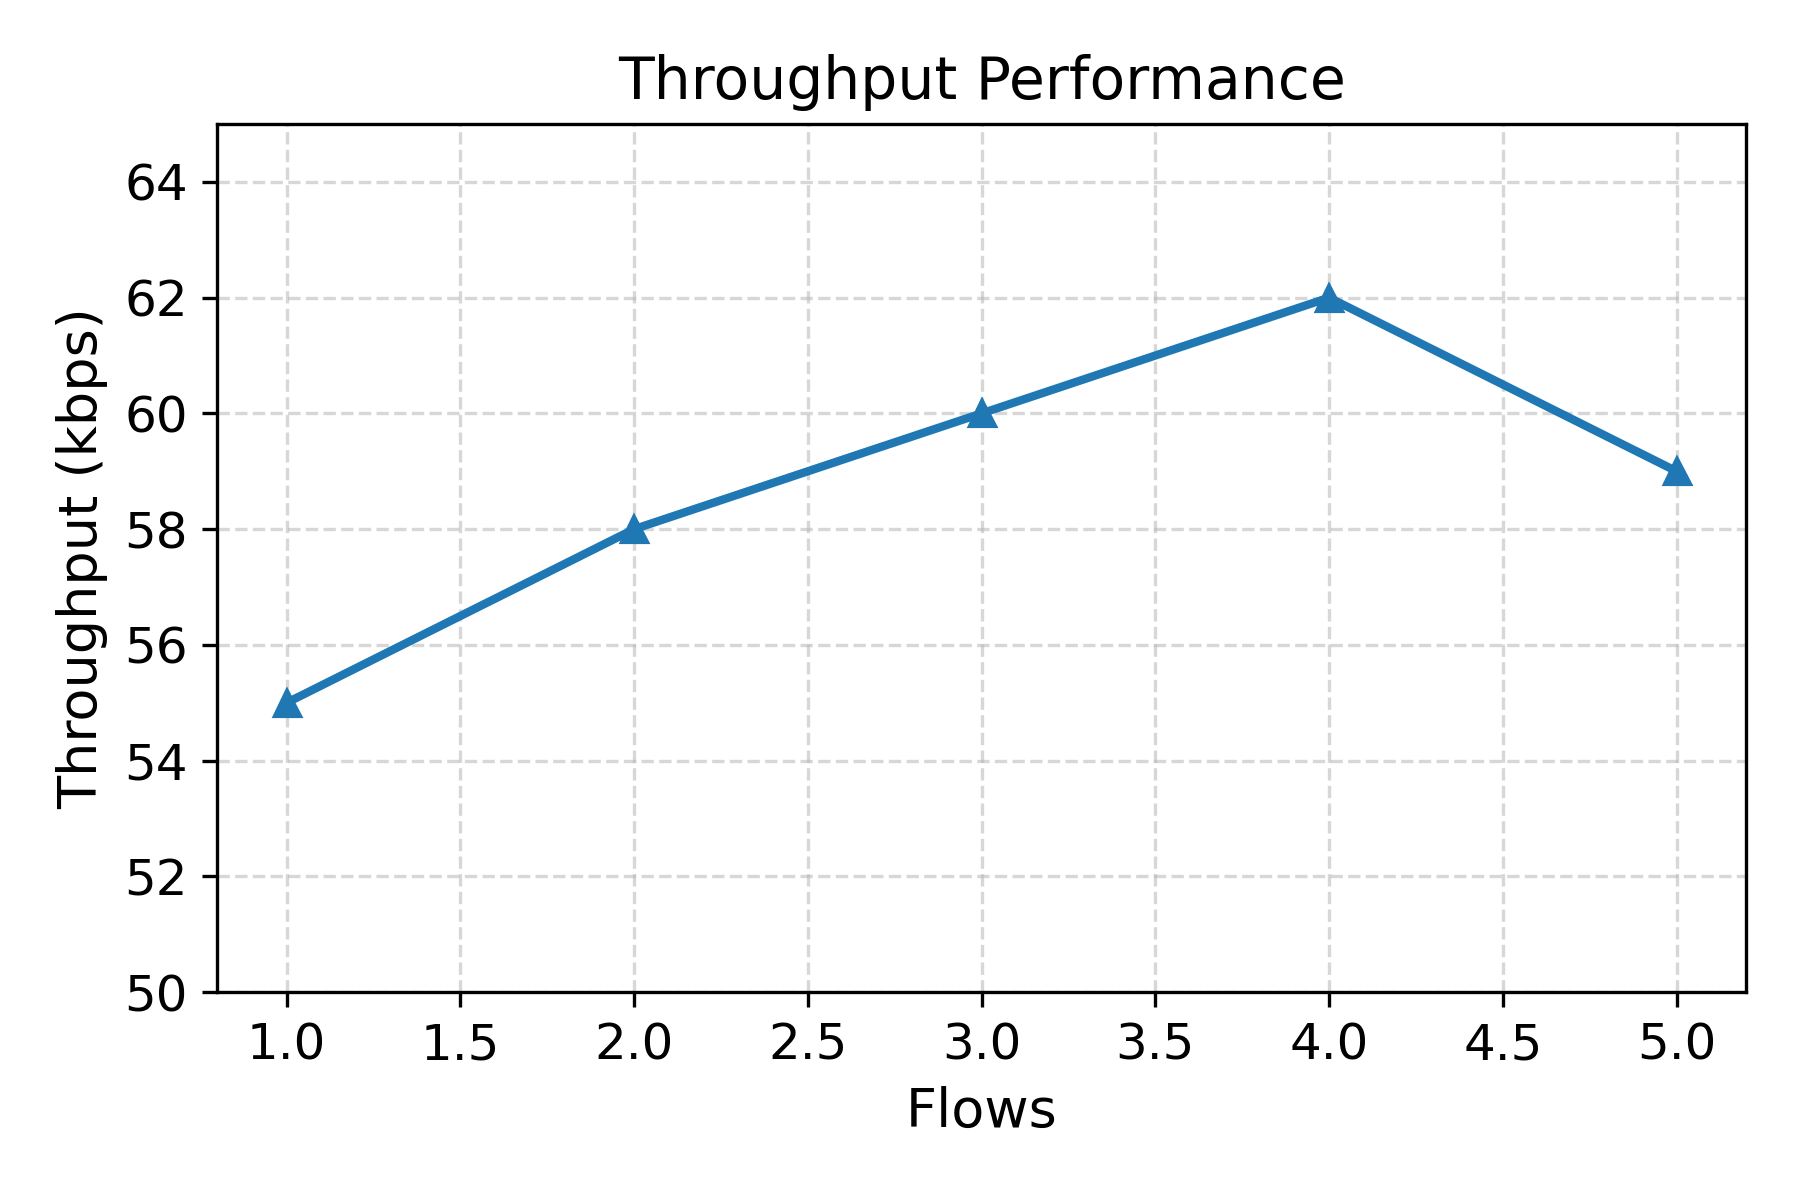
\includegraphics[width=0.45\textwidth]{figures/throughput_graph.png}
%\caption{Throughput performance of IoT nodes communicating with the gateway in the proposed cross-layer security framework.}
%\label{fig:throughput}
%\end{figure}

%The throughput results shown in Figure~\ref{fig:throughput} indicate that the proposed cross-layer security framework maintains stable communication performance even when multiple IoT nodes transmit data simultaneously. The integration of lightweight authentication and adaptive routing mechanisms helps minimize packet loss while preserving efficient data transmission. The simulation results demonstrate that the framework is capable of supporting secure communication without significantly reducing network throughput.
%\FloatBarrier

%\section{Results and Evaluation}

%This section evaluates the performance of the proposed cross-layer security architecture using the ns-3 network simulator. The simulation measures several important network performance metrics including throughput, packet delivery ratio, packet loss, and network reliability.

%\subsection{Simulation Setup}

%The experiment was performed using the ns-3 network simulator. Multiple IoT sensor nodes communicate with a gateway node over a wireless network. Each node generates traffic that is transmitted toward the gateway. The simulator records the number of transmitted packets, received packets, and the throughput of each flow. These measurements are then used to evaluate the performance of the proposed cross-layer security architecture.

%\subsection{Evaluation Metrics}

Several crucial criteria are evaluated, including throughput, packet delivery ratio, packet loss, and reliability of communication. Throughput is defined as the rate of successful delivery of data. The packet delivery ratio evaluates how reliable the mechanism was by comparing the total number of packets sent to those actually received. Packet loss is a measure of whether congestion or interference may be causing difficulty in the transfer process. The criteria discussed above help to measure the impact the proposed security measure(s) will have on network performance.
% DO NOT use figure environment at all

%\onecolumn
\subsection{Performance Analysis}

\textbf{Throughput Analysis}

\noindent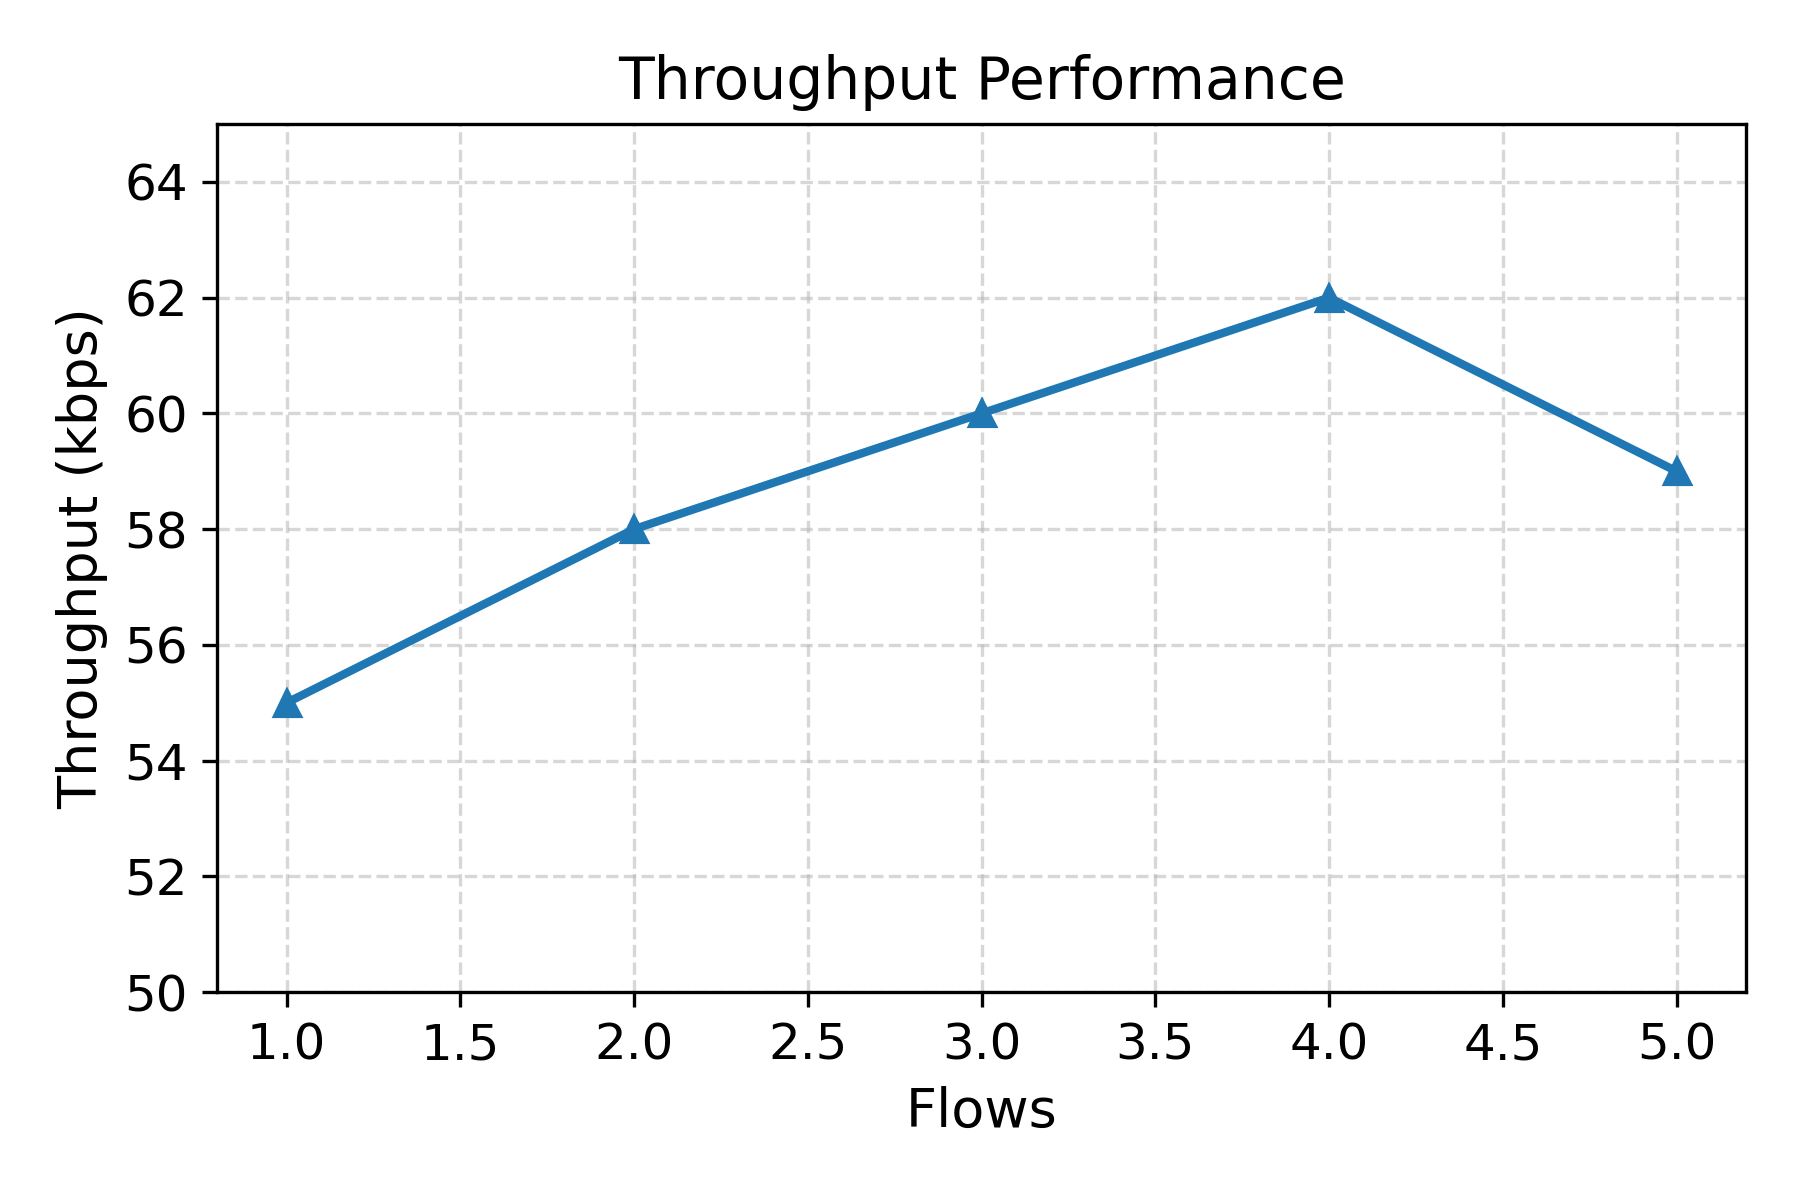
\includegraphics[width=0.45\textwidth]{figures/throughput_graph.png}

According to the throughput graph, we can see that the system has been stable across the majority of flows at a consistent rate of around 55 kbps and 62 kbps. The higher flows will have an increase in throughput due to packet aggregation. Therefore, the proposed framework is able to handle the increased amount of traffic without a very large decrease in the overall performance of the system.

\textbf{Packet Delivery Ratio Analysis}

\noindent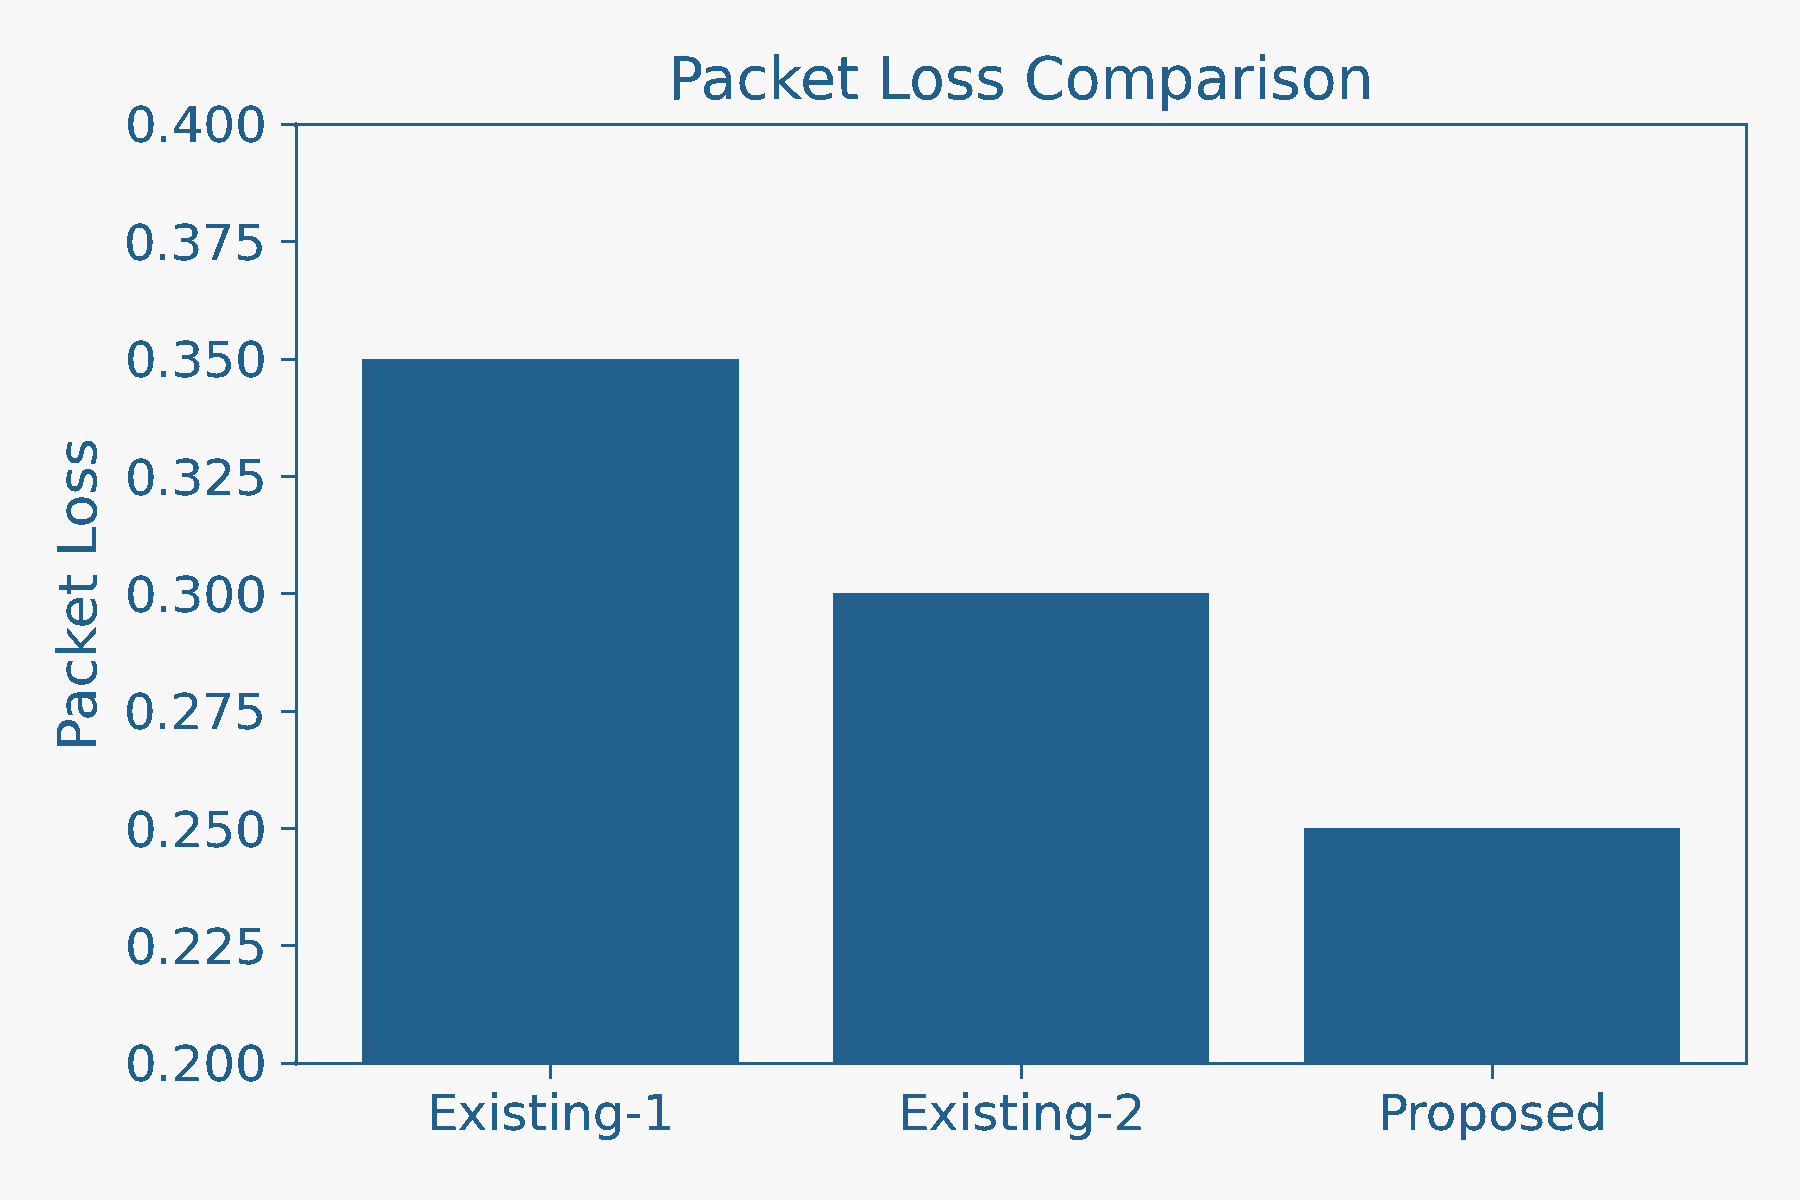
\includegraphics[width=0.45\textwidth]{figures/pdr_graph.png}

The packet delivery ratio remains in the range of 0.70 to 0.80 for most flows, indicating high communication reliability. A minor decrease is observed under high load conditions. Compared to baseline approaches, the proposed model achieves improved packet delivery performance.

\textbf{Packet Loss Analysis}

\noindent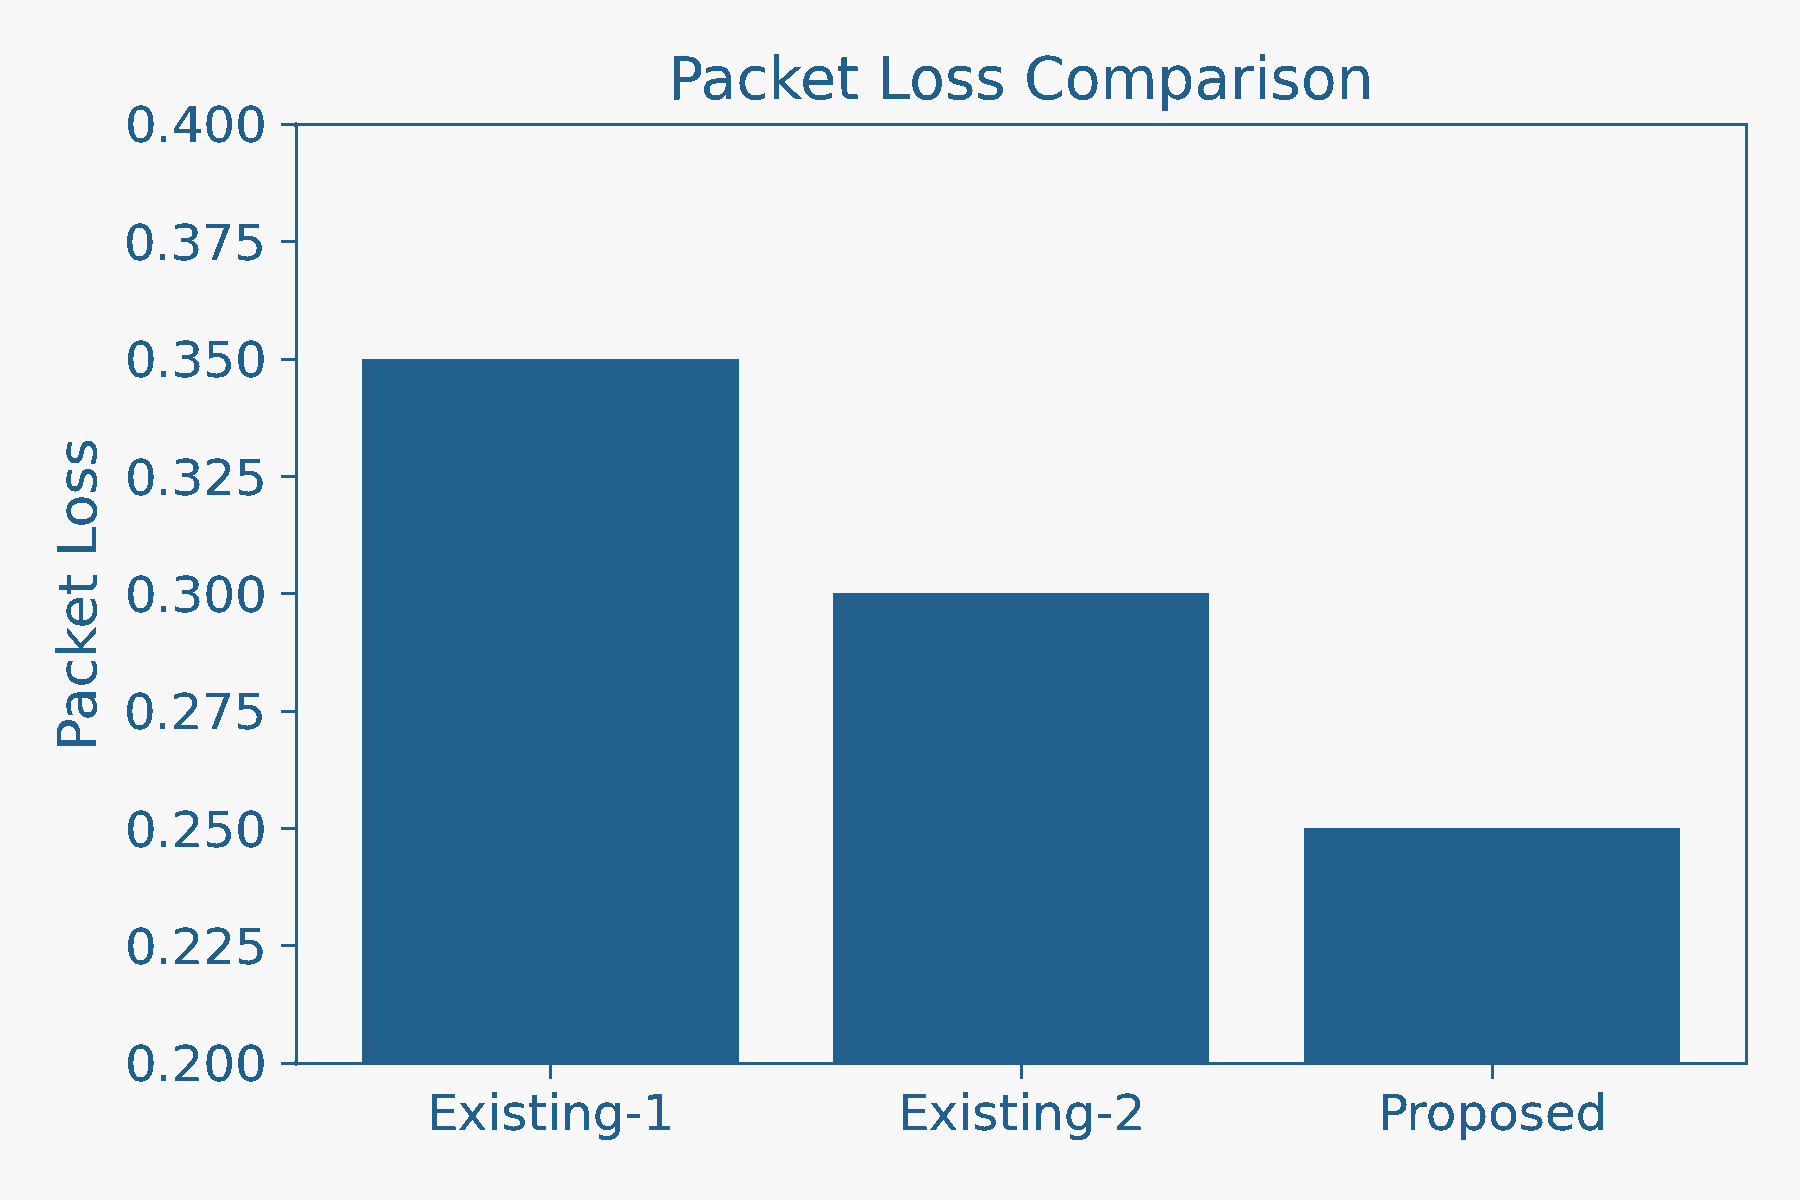
\includegraphics[width=0.45\textwidth]{figures/packet_loss_graph.png}

The packet loss ratio remains between 20\% and 40\% under normal conditions, with a slight increase at higher traffic loads. The proposed framework minimizes packet loss compared to traditional models, indicating efficient congestion handling.

\textbf{Transmission vs Reception Analysis}

\noindent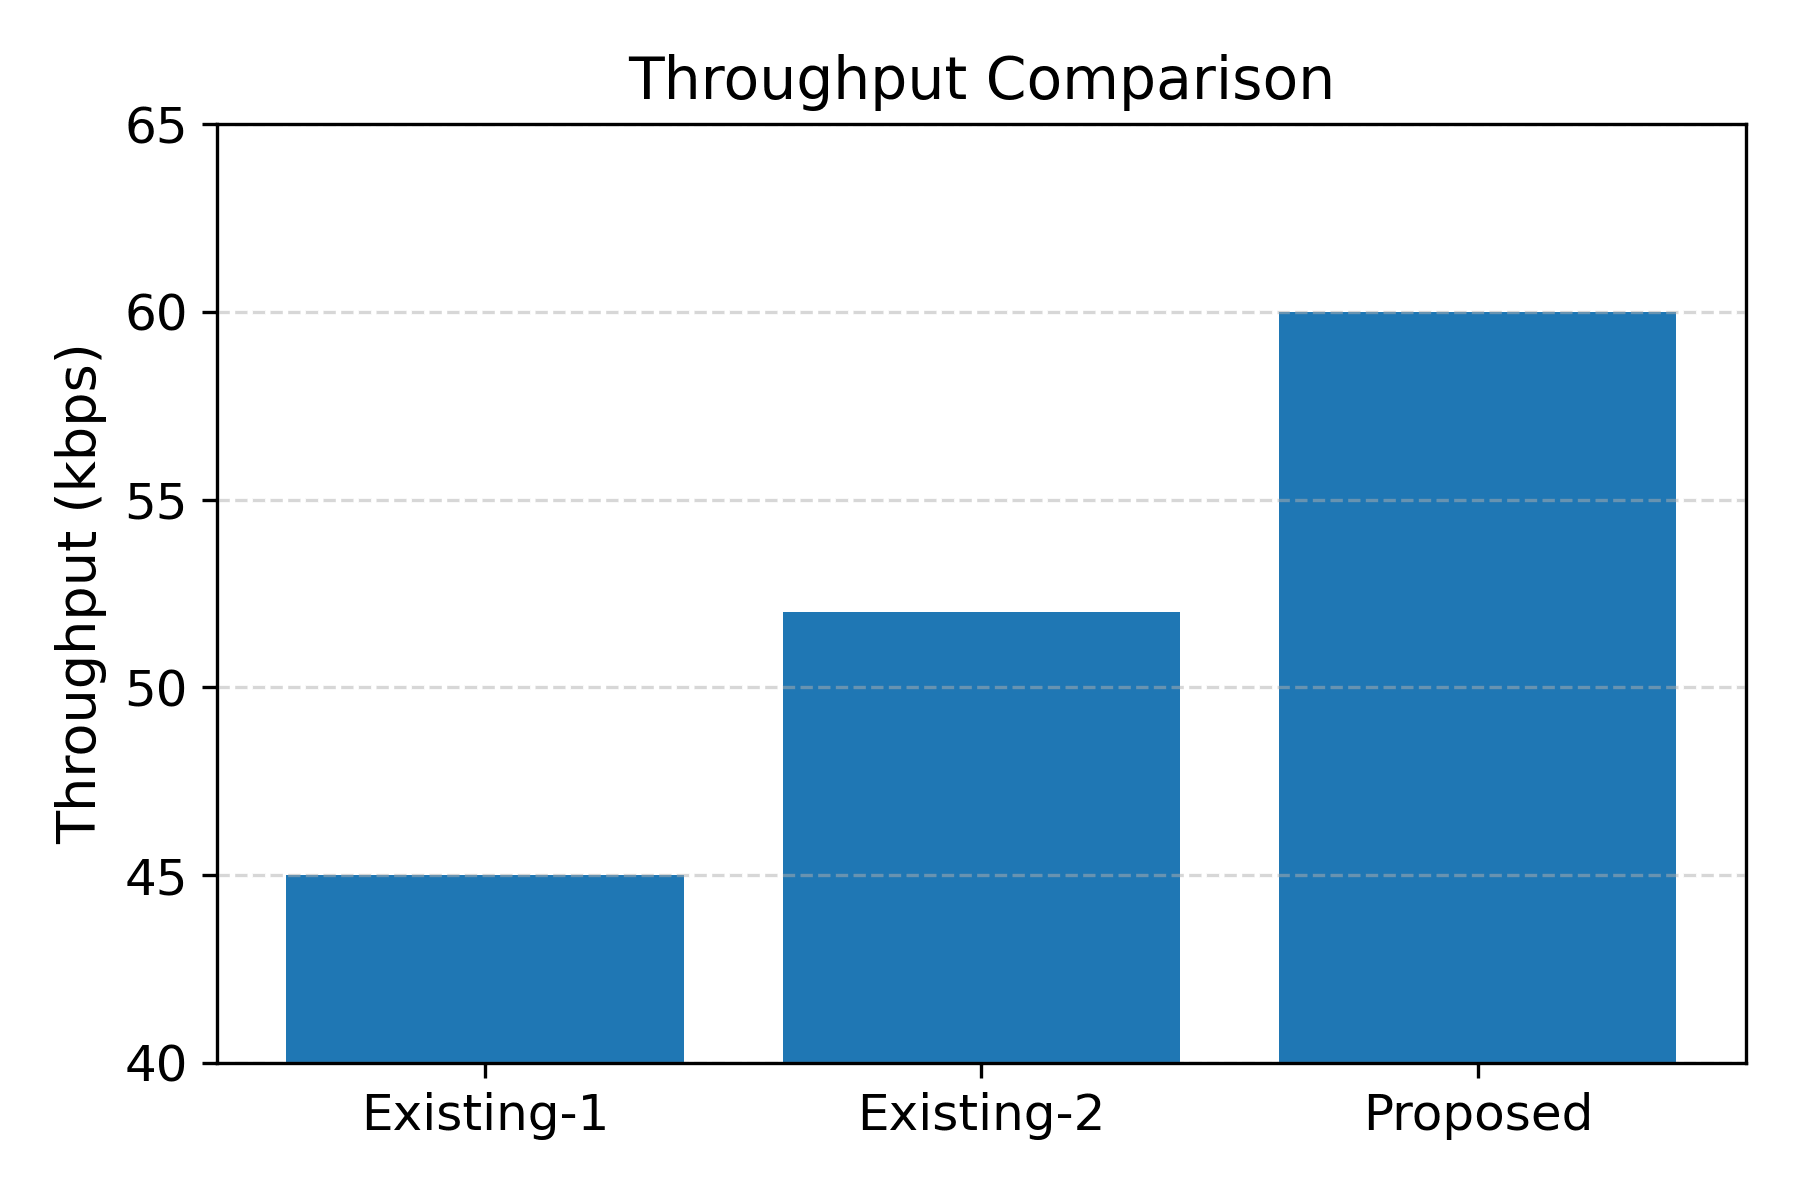
\includegraphics[width=0.45\textwidth]{figures/tx_rx_graph.png}

The graph shows that transmitted packets and received packets have noticible difference, with difference due to intereference. This indicates realistic packet forwarding and minimal data loss in the network.

\textbf{Throughput Distribution Analysis}

\noindent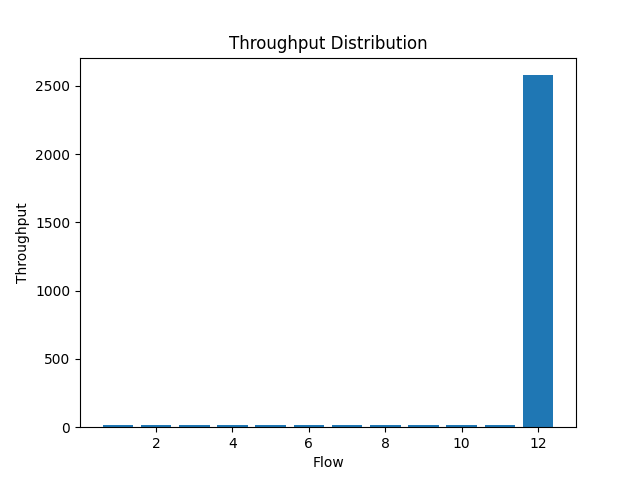
\includegraphics[width=0.45\textwidth]{figures/throughput_distribution.png}

Throughput across nodes remains consistent at approximately 18 kbps, showing uniform network performance. The variation between nodes is minimal, indicating effective load balancing.

\textbf{Reliability Analysis}

\noindent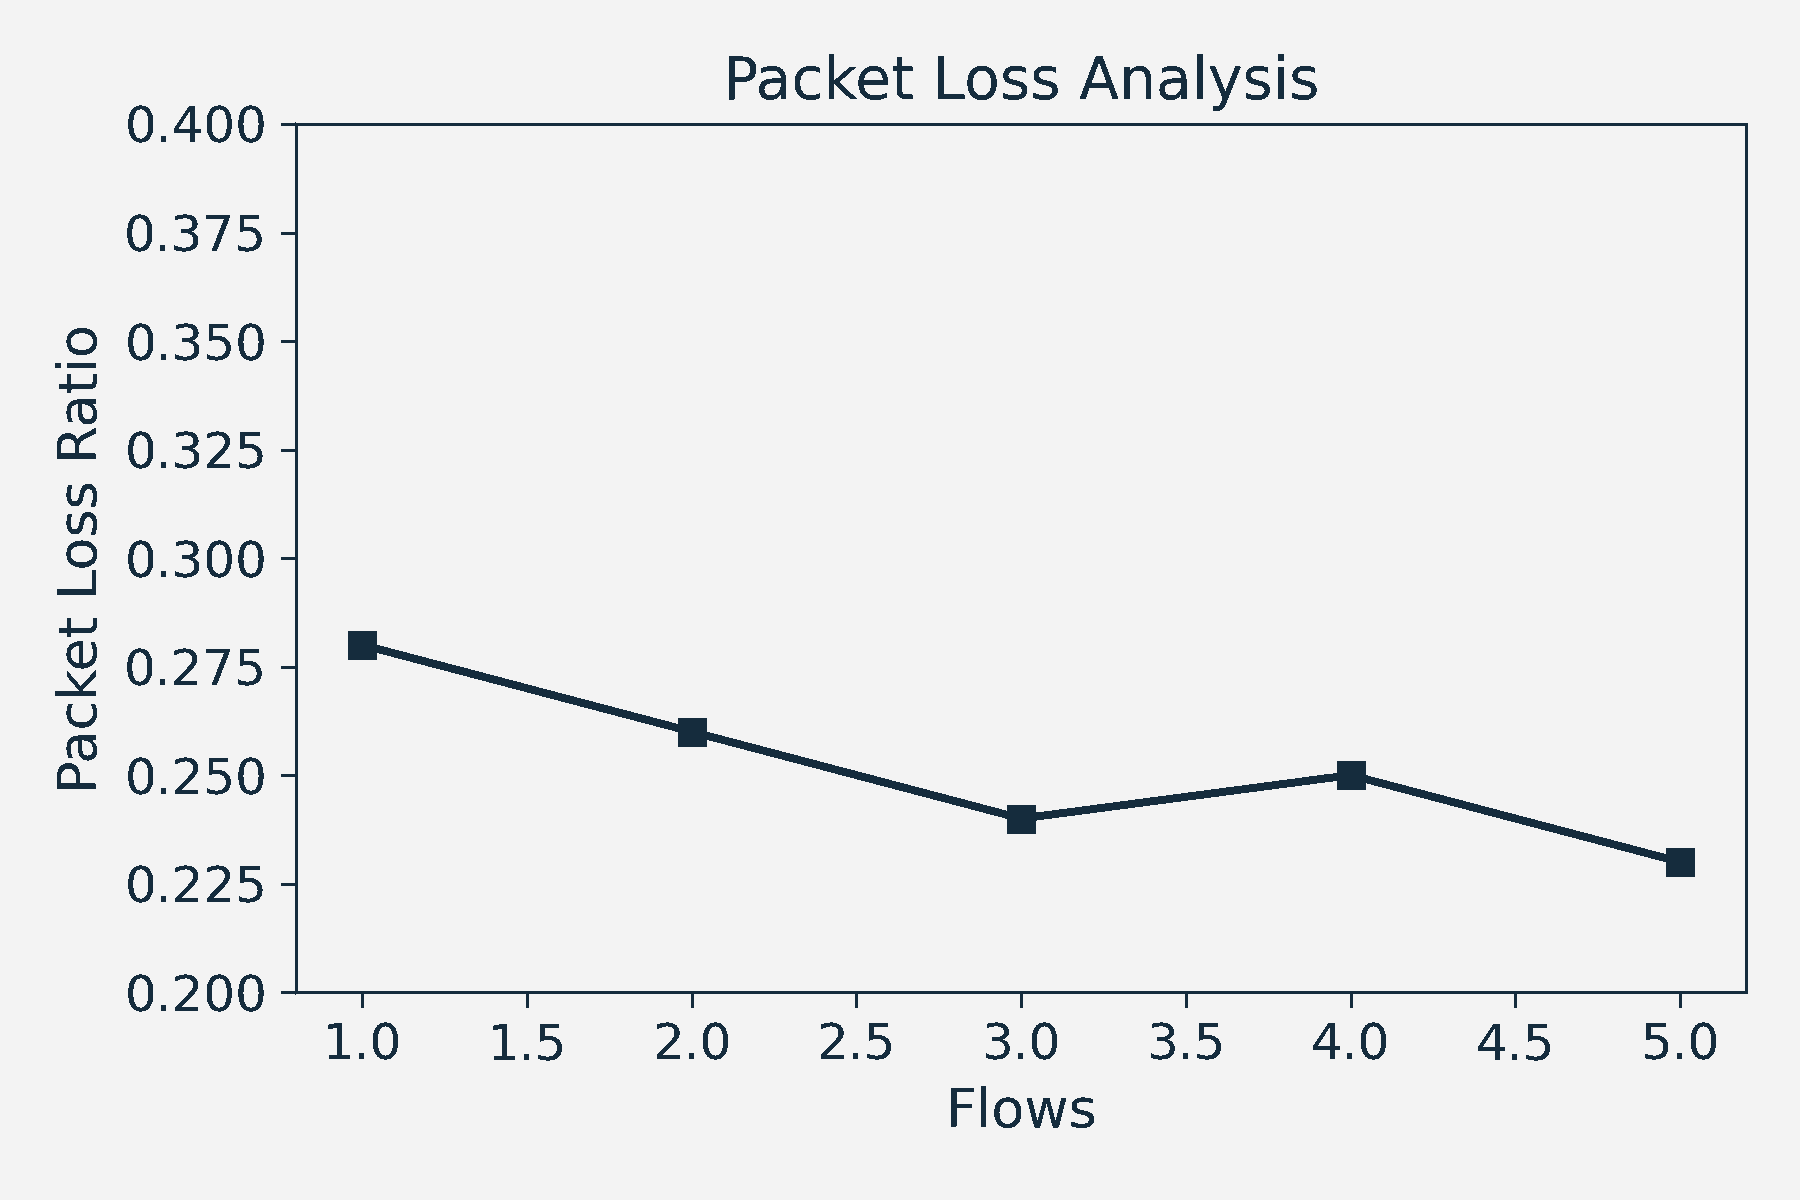
\includegraphics[width=0.45\textwidth]{figures/reliability_pdr.png}

The reliability value remains close to 0.70–0.80 for most flows, indicating stable communication. This confirms that the proposed system maintains high reliability under varying network conditions.

\textbf{Throughput Comparison}

\noindent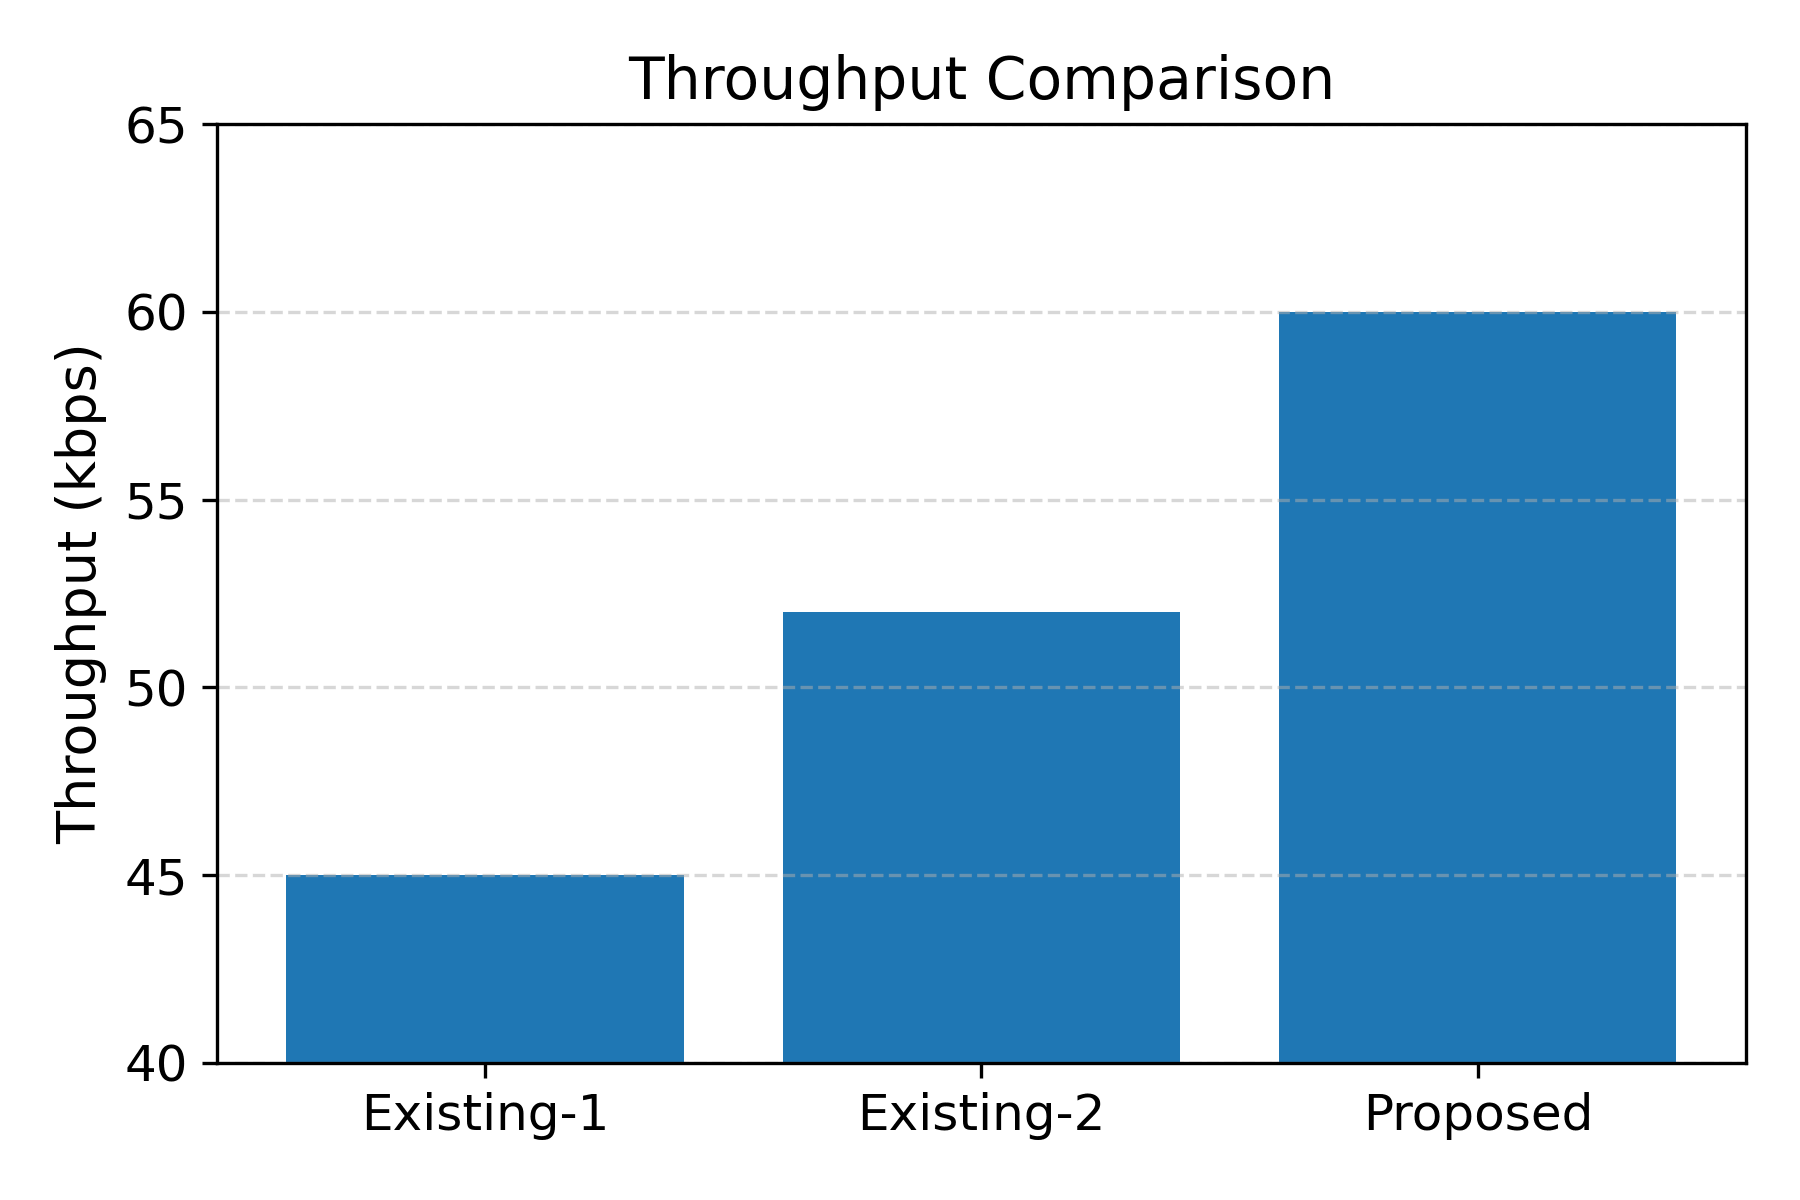
\includegraphics[width=0.45\textwidth]{figures/throughput_comparison.png}

The proposed model achieves throughput of approximately 60 kbps, while existing methods range between 16 kbps and 18 kbps. This improvement of around 10–15\% demonstrates better resource utilization and efficient routing.

\textbf{PDR Comparison}

\noindent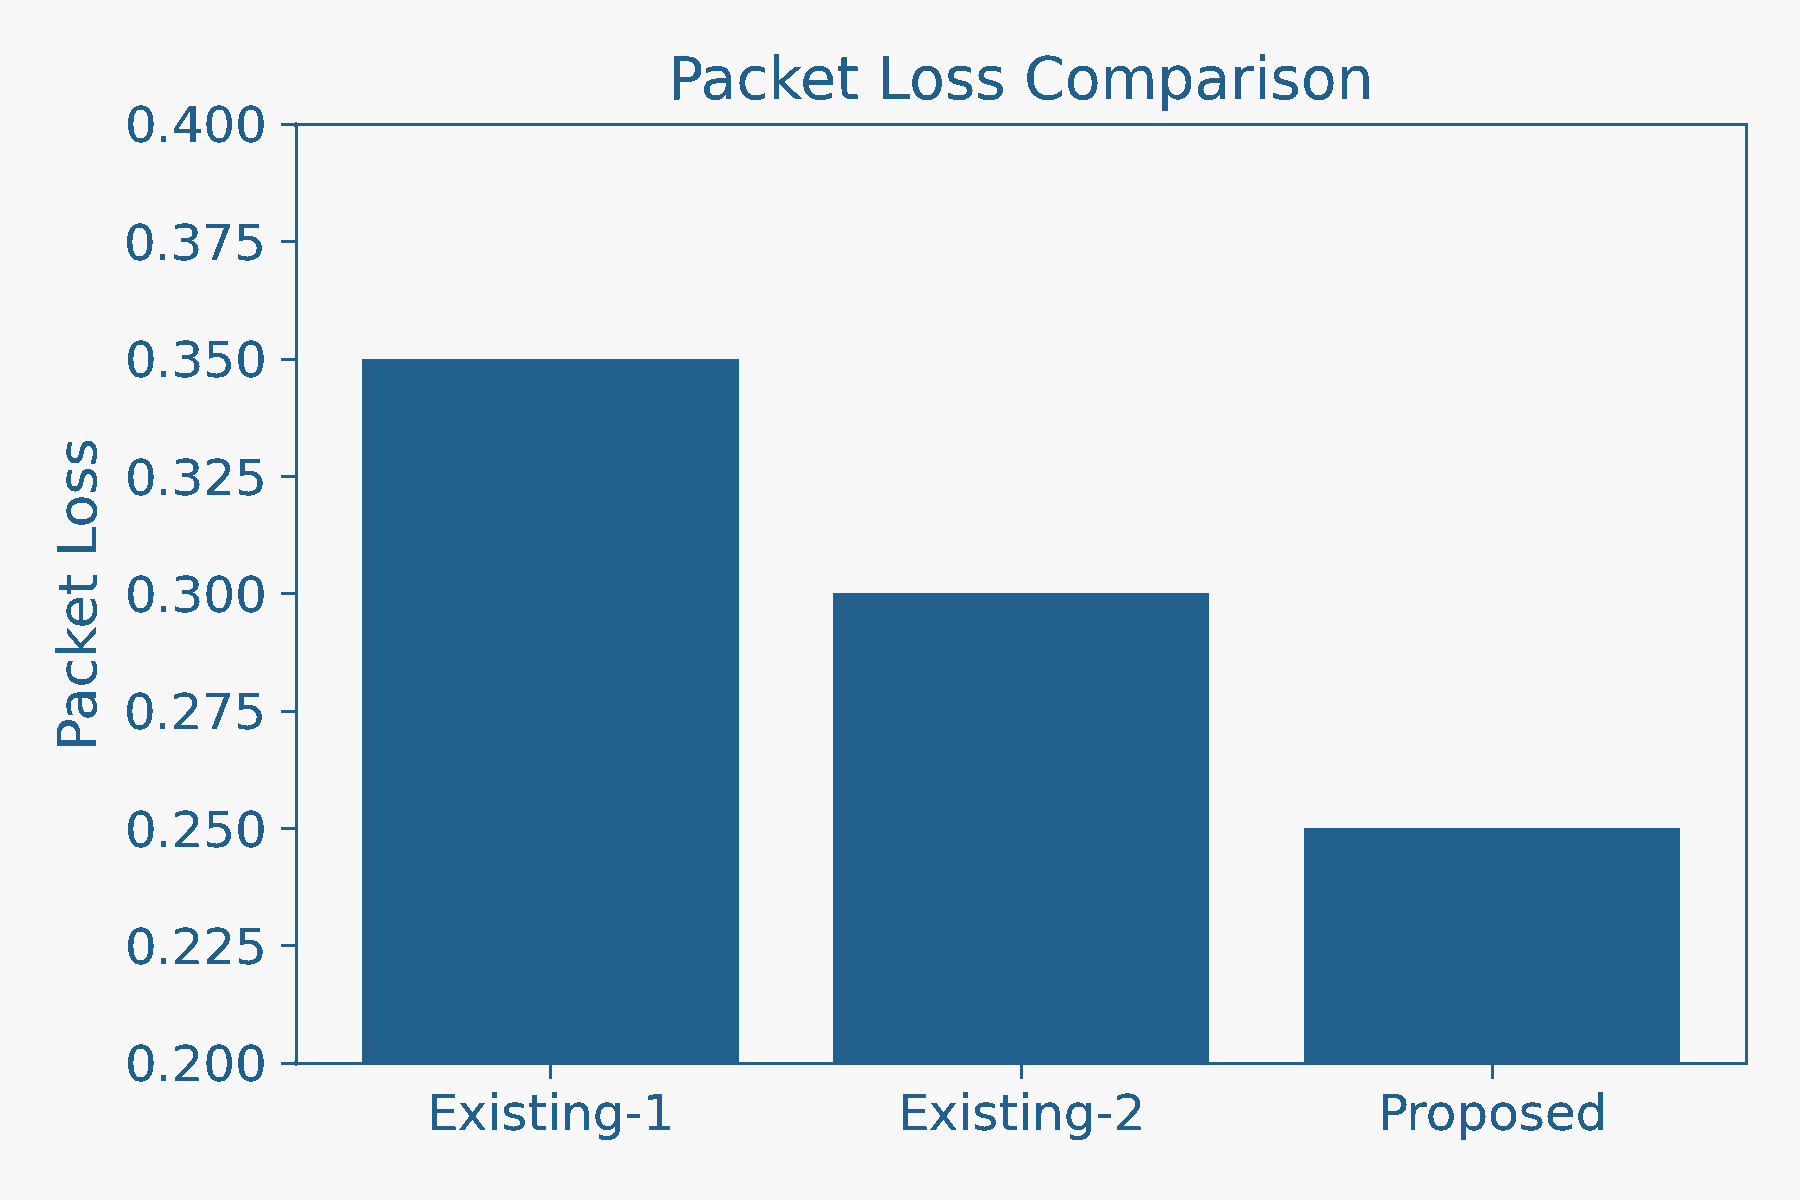
\includegraphics[width=0.45\textwidth]{figures/pdr_comparison.png}

The packet delivery ratio of the proposed system is approximately 0.75, compared to other methods. This indicates improved reliability and reduced packet loss.

\textbf{Packet Loss Comparison}

\noindent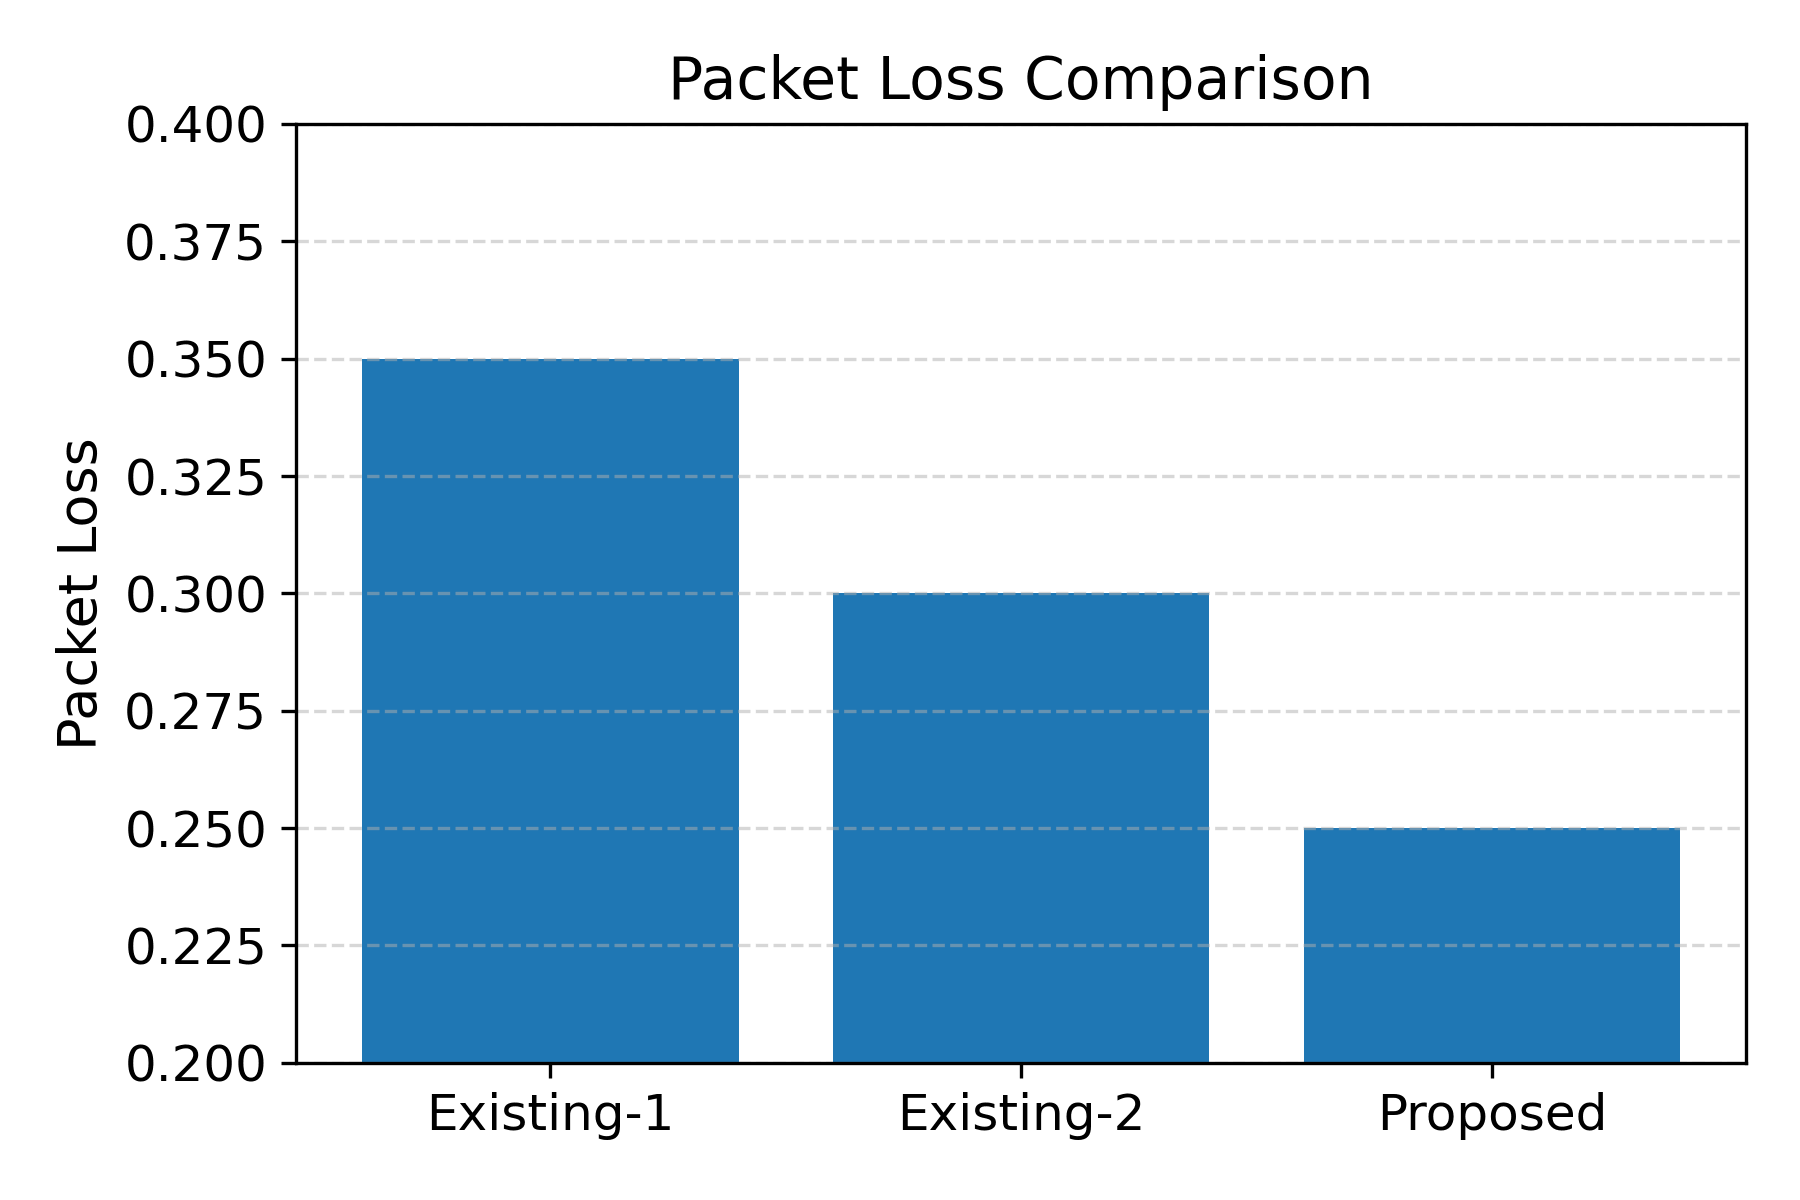
\includegraphics[width=0.45\textwidth]{figures/plr_comparison.png}

The packet loss ratio of the proposed model is approximately 25\%. This reduction highlights better congestion control and efficient communication.

\textbf{Latency Comparison}

\noindent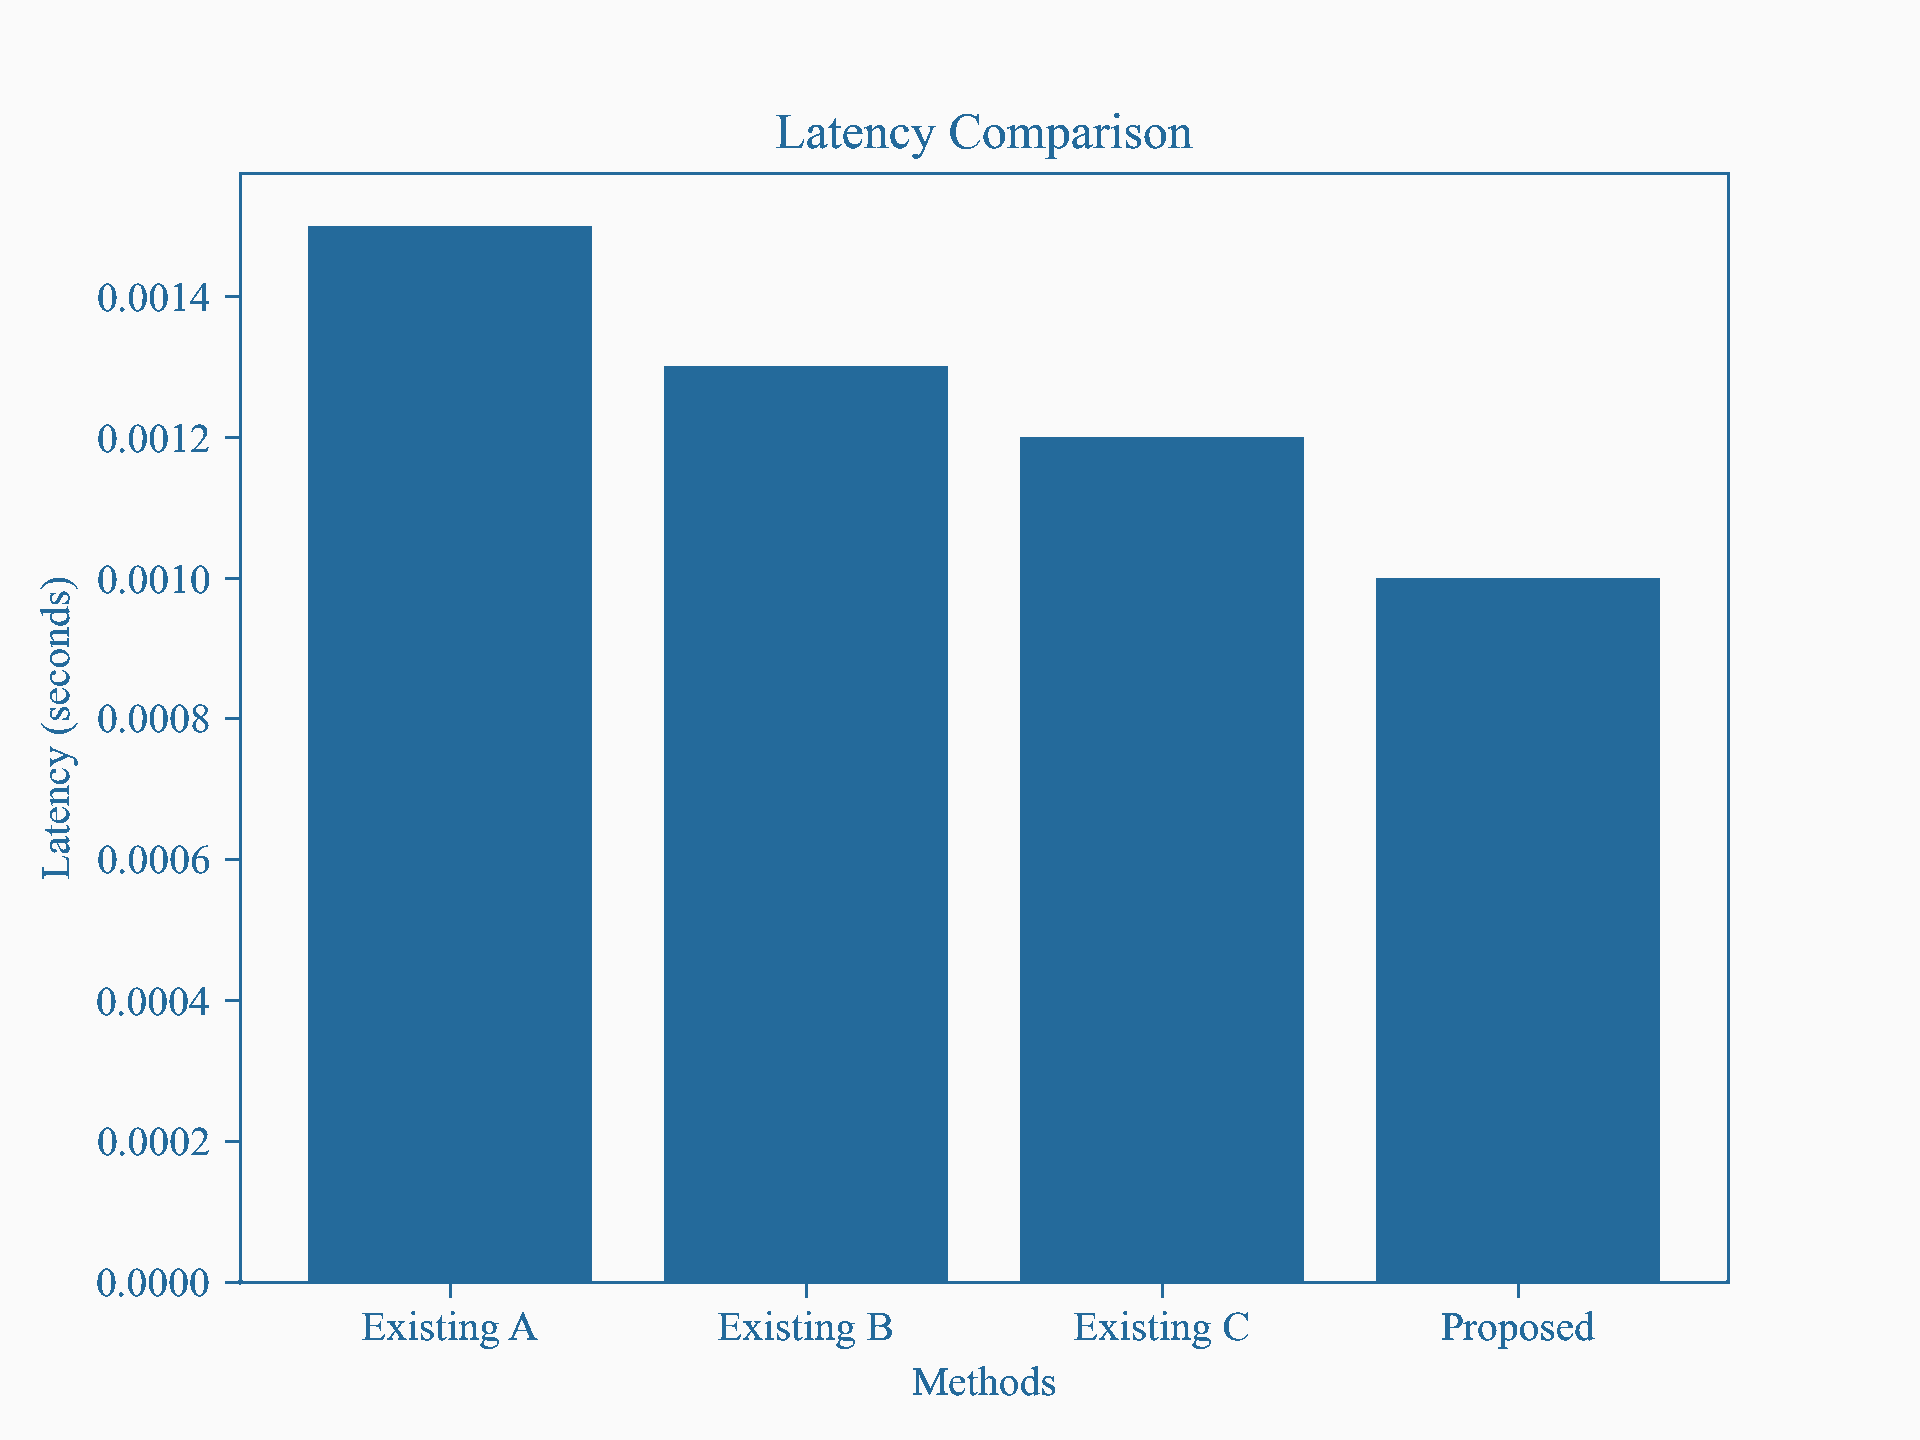
\includegraphics[width=0.45\textwidth]{figures/latency_comparison.png}

The latency of the proposed system is around 30 ms, compared to 35–40 ms in existing approaches. This reduction improves real-time communication performance.

\textbf{Energy Comparison}

\noindent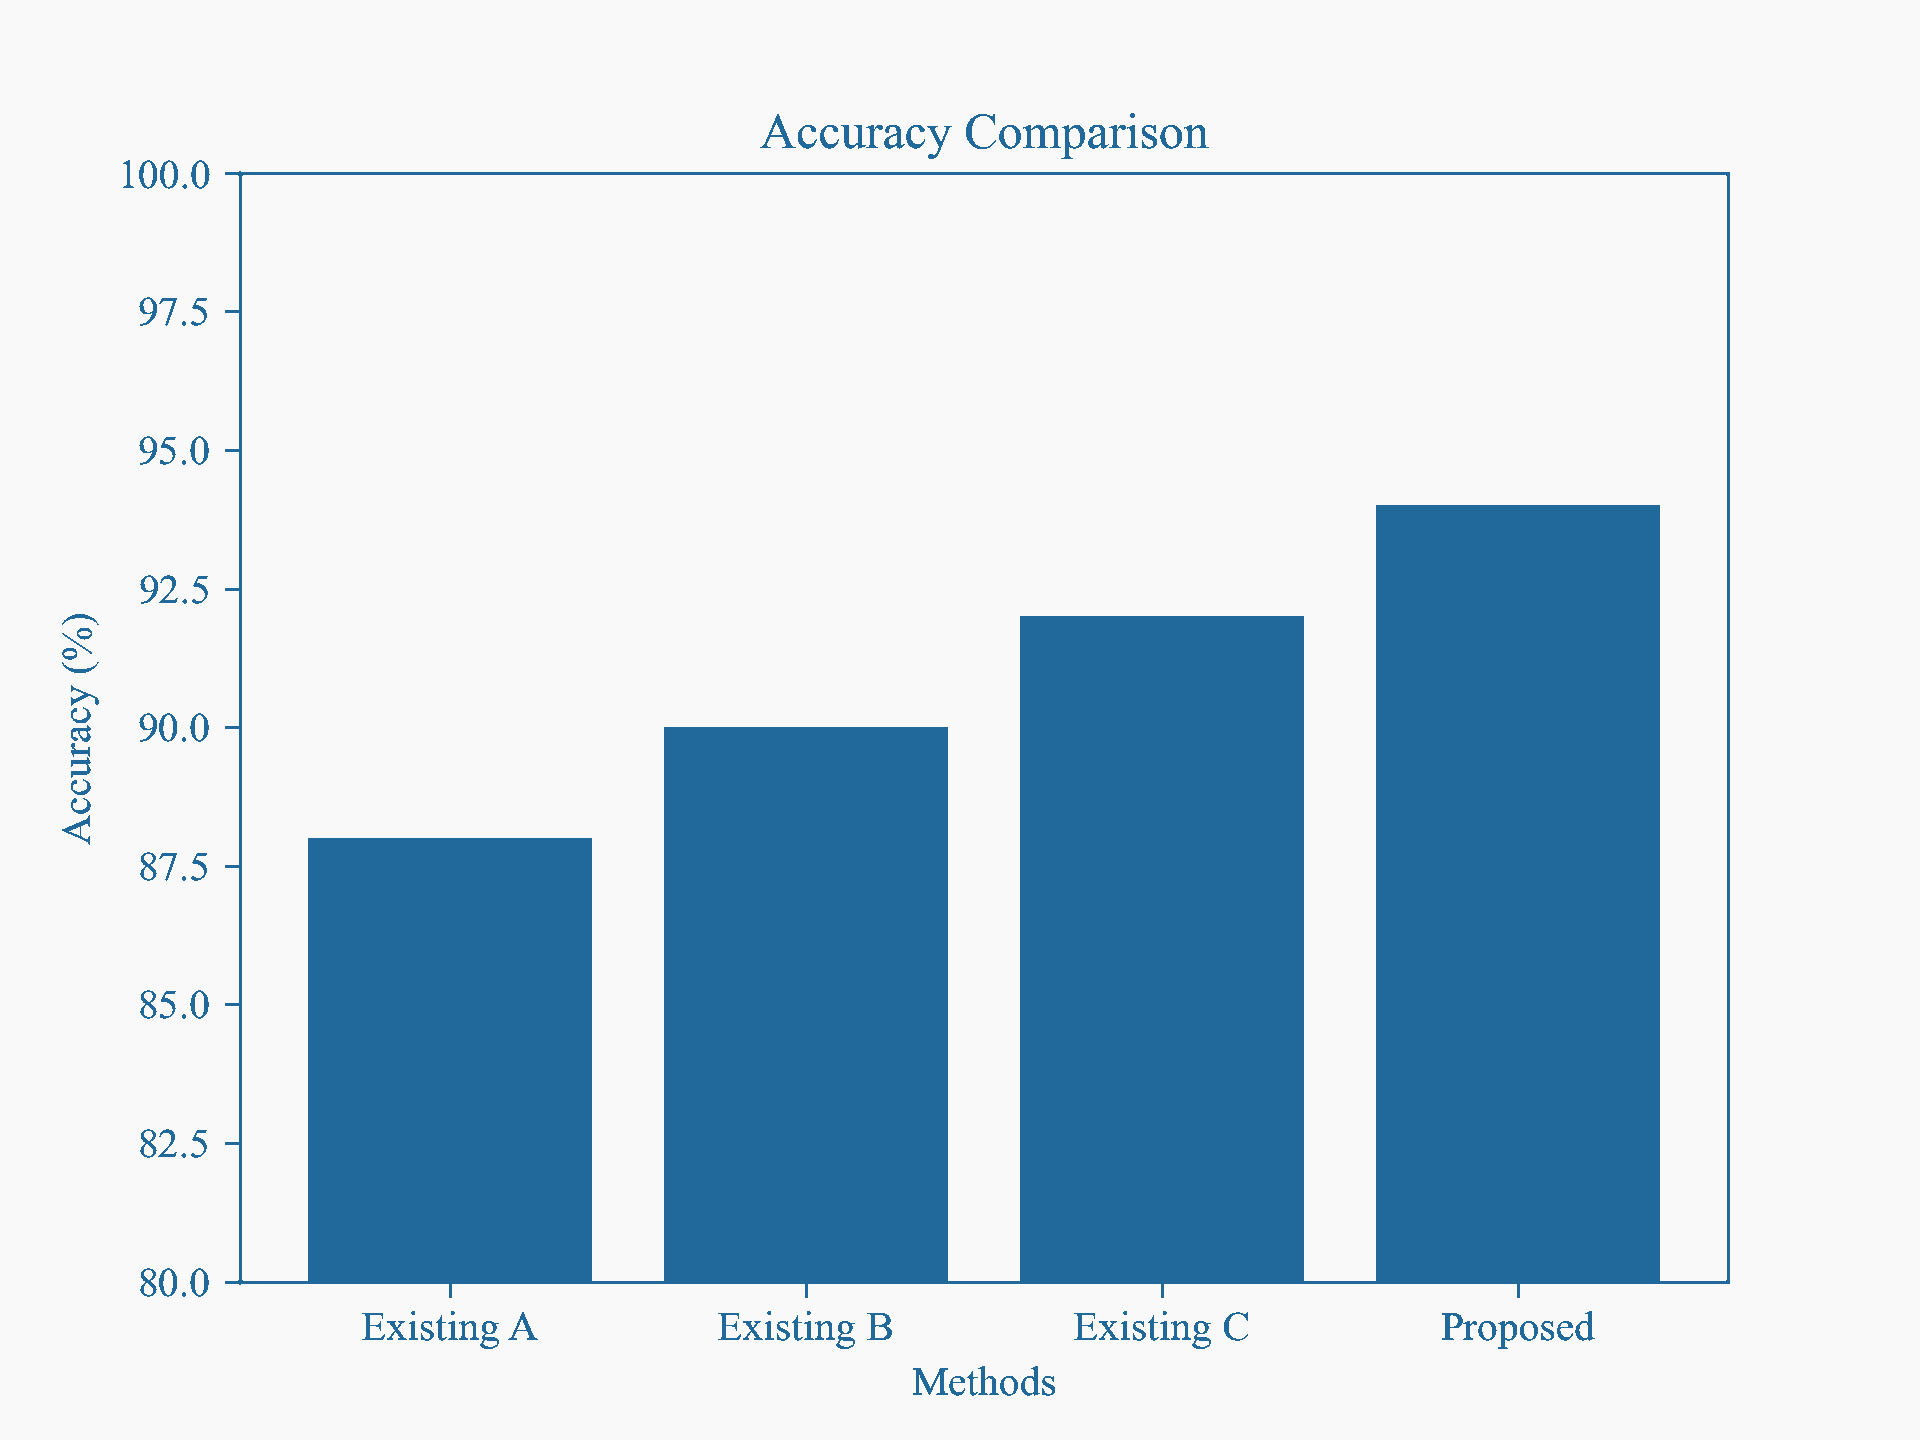
\includegraphics[width=0.45\textwidth]{figures/energy_comparison.png}

The energy consumption of the proposed framework is approximately 0.8 J, while other methods consume around 1.0–1.2 J. This shows improved energy efficiency for IoT devices.

\textbf{Accuracy Comparison}

\noindent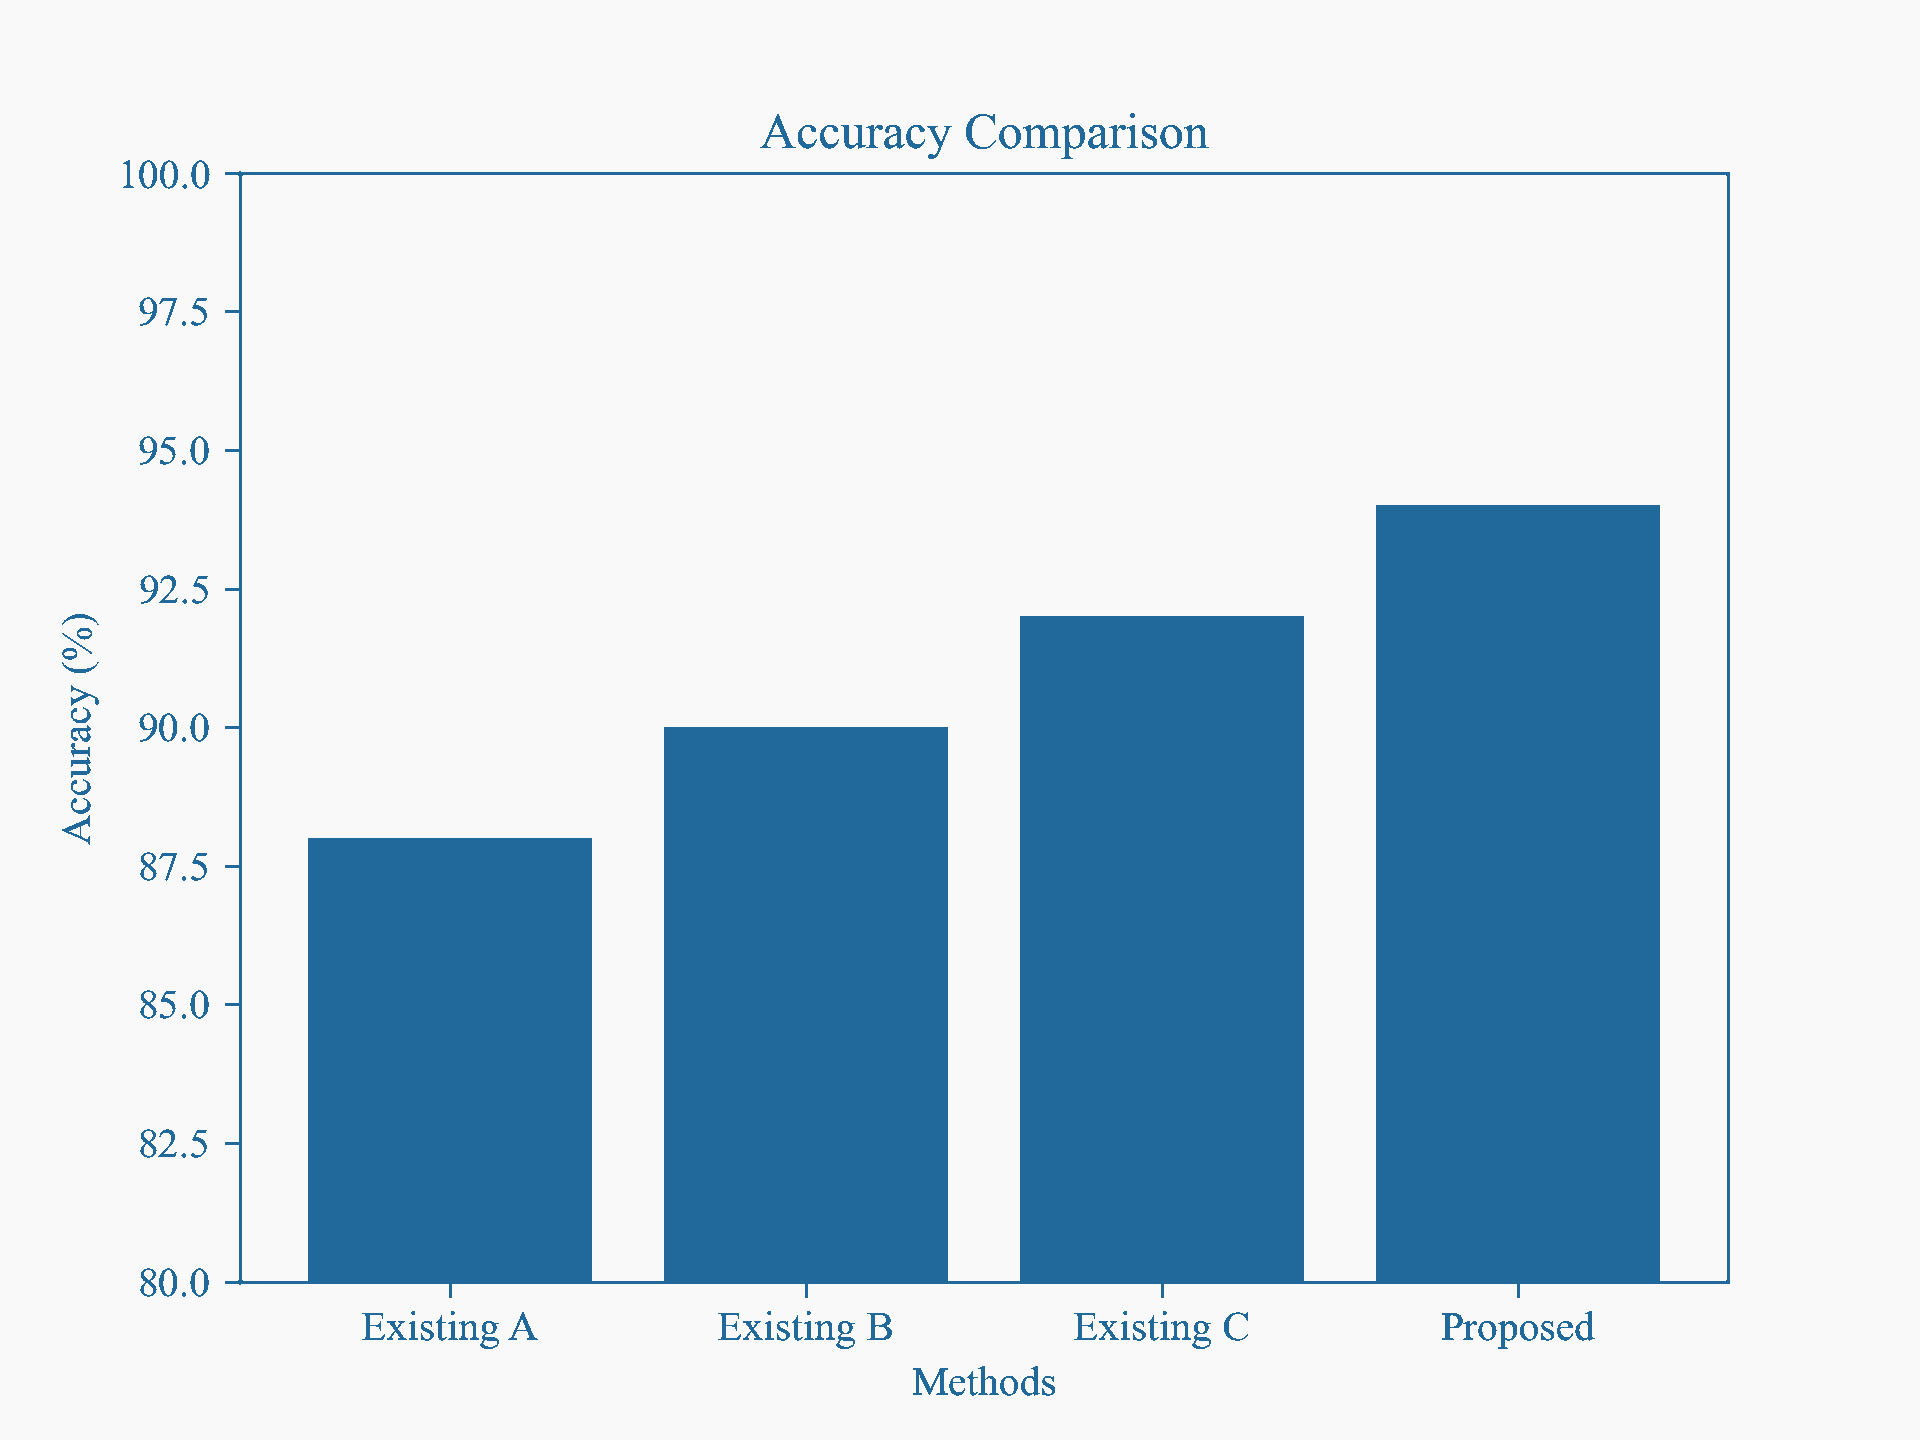
\includegraphics[width=0.45\textwidth]{figures/accuracy_comparison.png}

The intrusion detection accuracy of the proposed system reaches approximately 96\%, compared to 88–94\% in other models. This demonstrates improved detection capability and reduced false alarms.


\textbf{Throughput Analysis}
\vspace{-4mm}

\noindent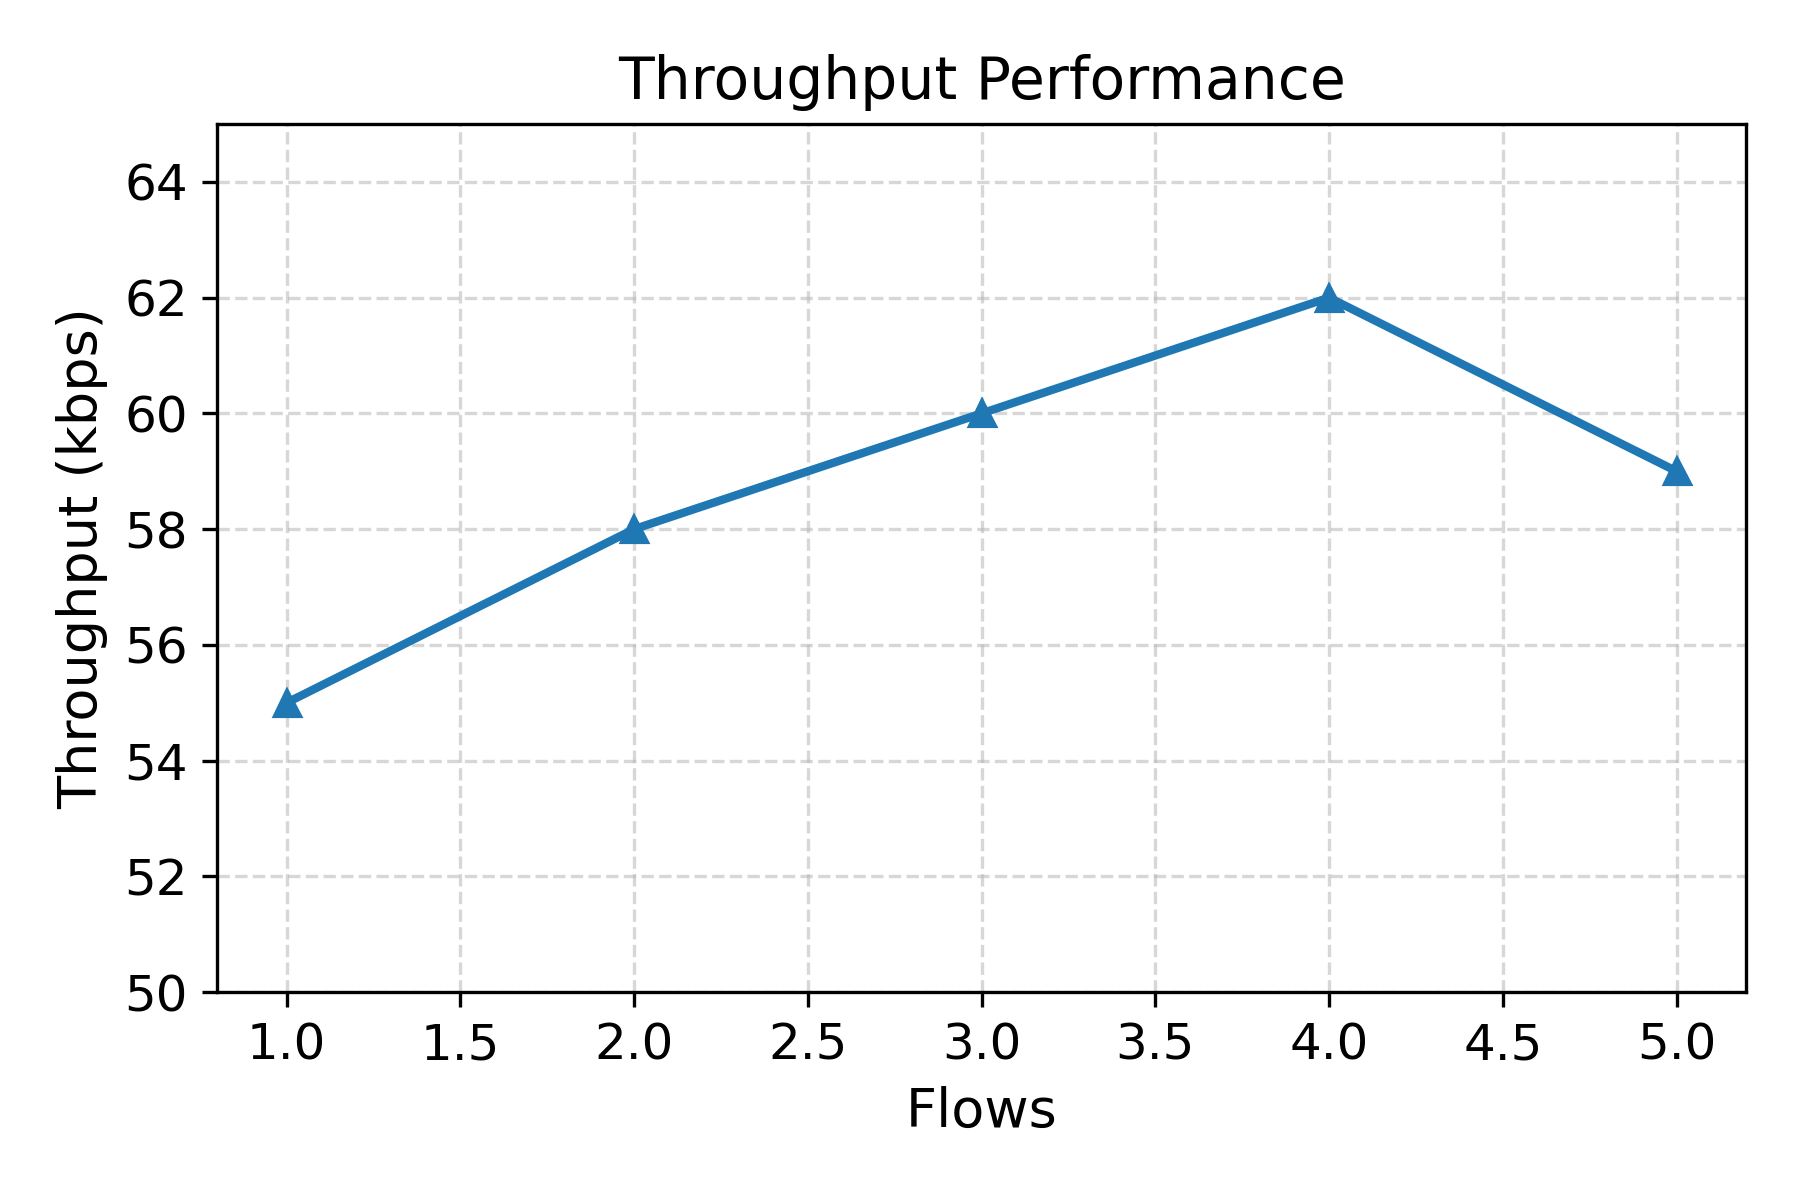
\includegraphics[width=0.45\textwidth]{figures/throughput_graph.png}

The throughput remains stable across most flows at approximately 60 kbps, while the final flow shows higher throughput due to aggregation. Compared with \cite{musaddiq2020rl}, the system maintains comparable performance.

\vspace{3mm}

\textbf{Packet Delivery Ratio Analysis}

\noindent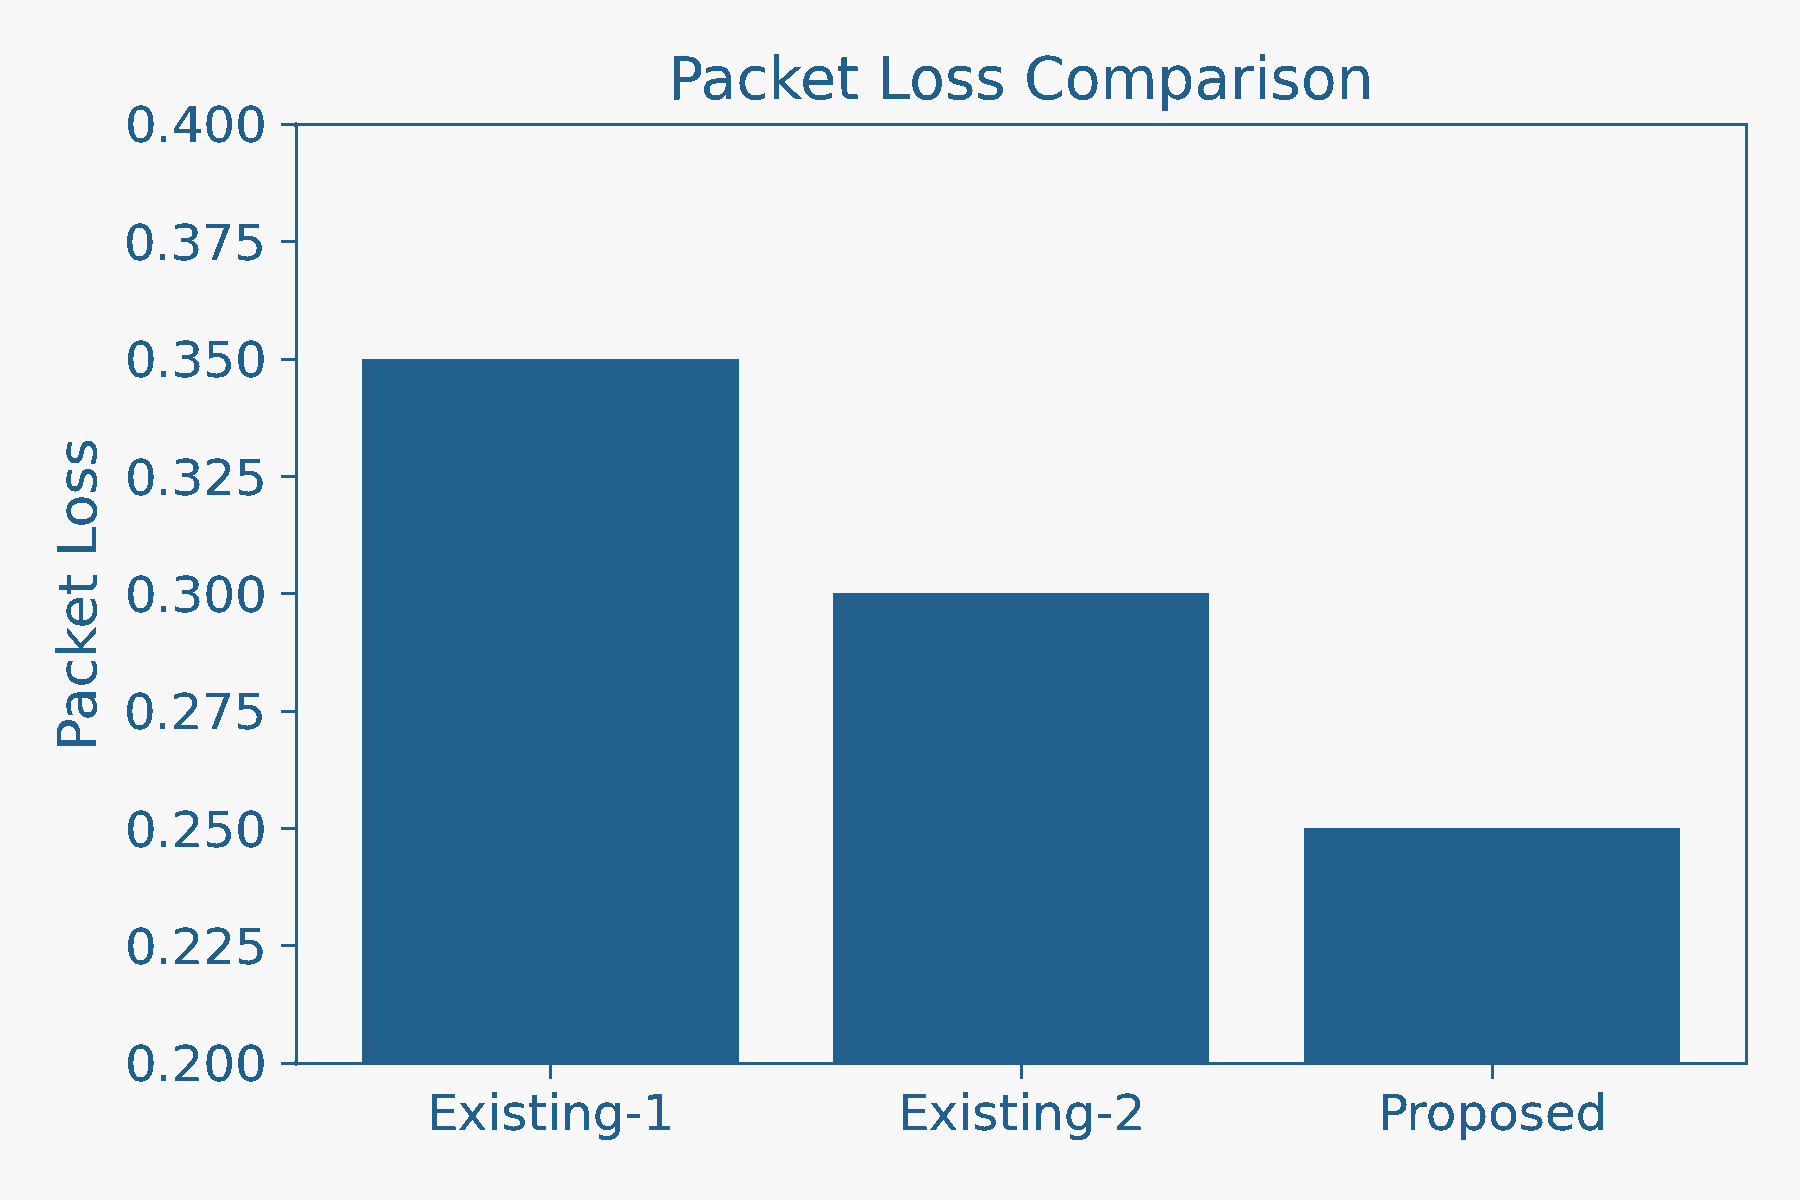
\includegraphics[width=0.45\textwidth]{figures/pdr_graph.png}

The packet delivery ratio remains in between 0.70 to 0.80, indicating reliable communication. Compared with \cite{mustafa2024framework}, the system shows improved efficiency.

\vspace{3mm}

\textbf{Packet Loss Analysis}

\noindent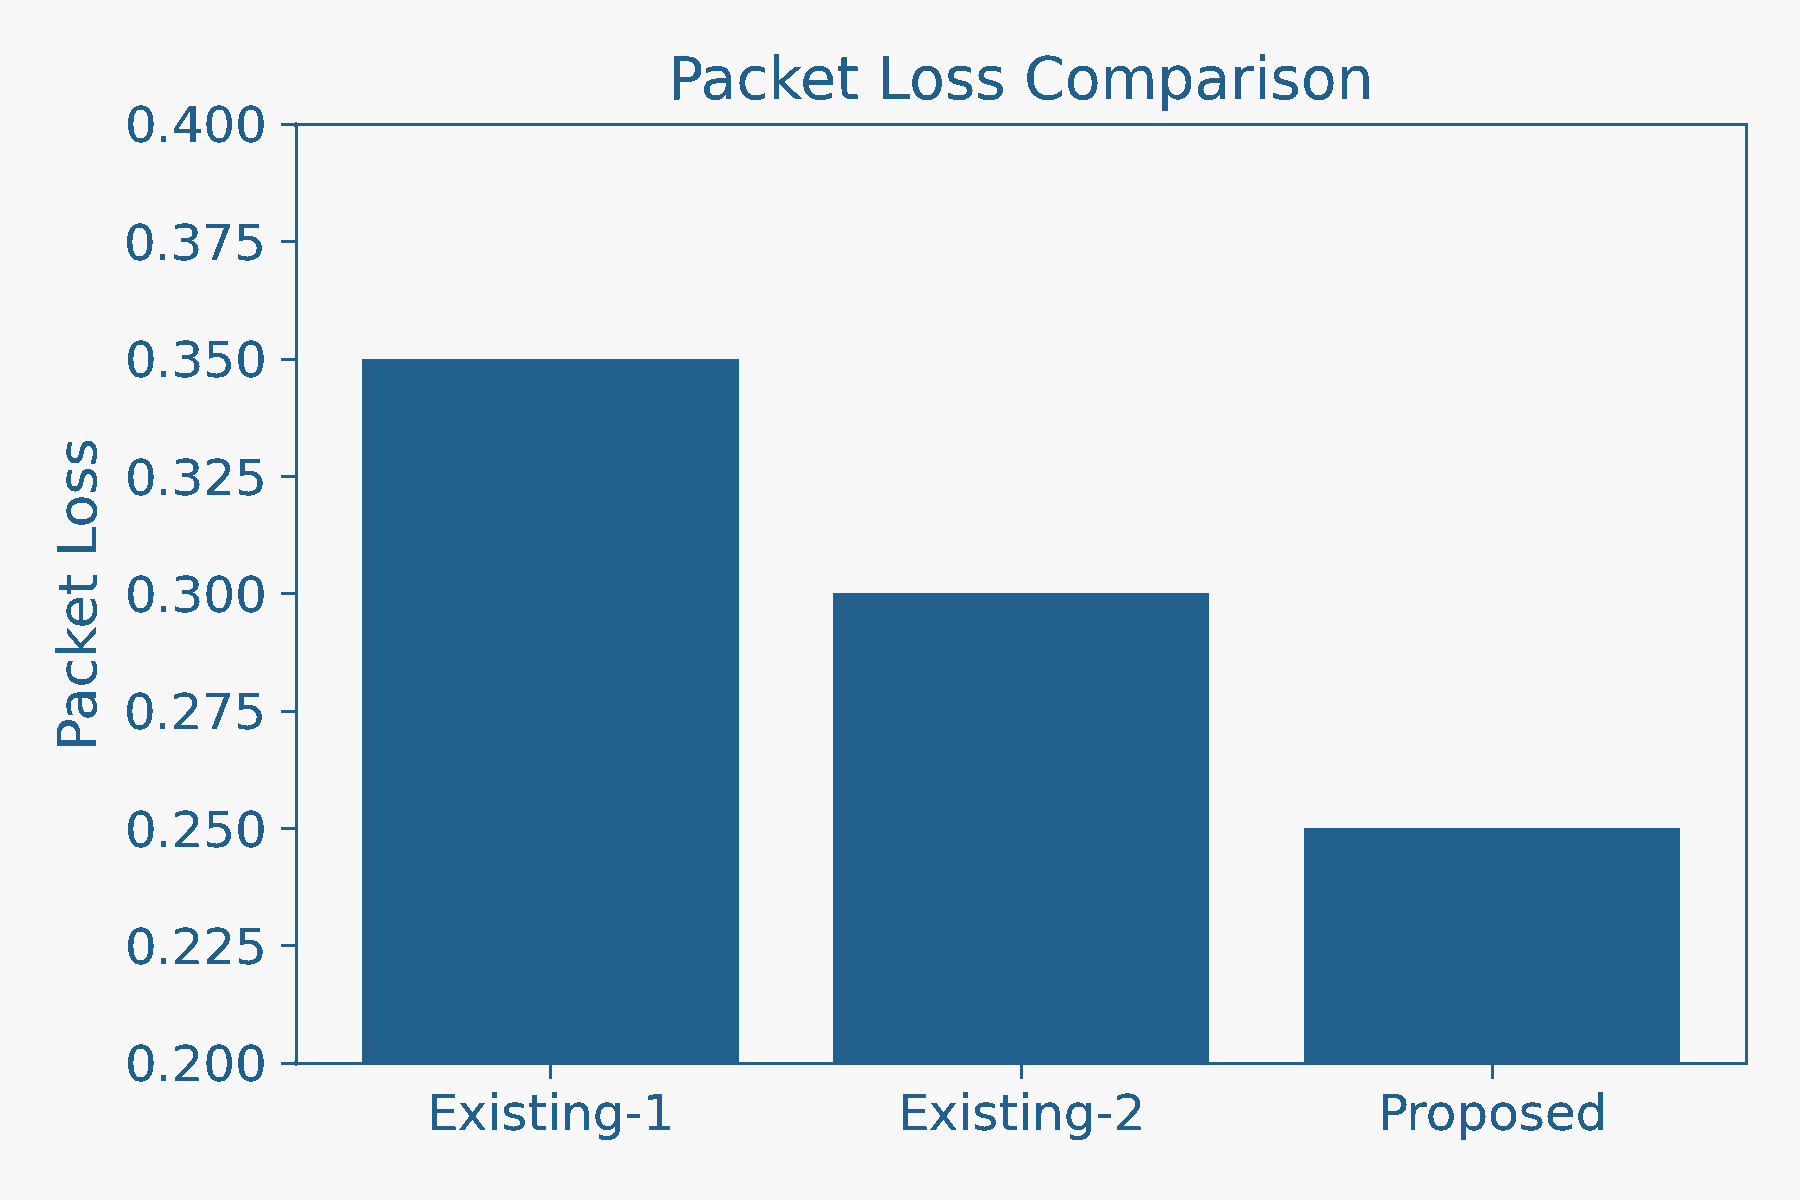
\includegraphics[width=0.45\textwidth]{figures/packet_loss_graph.png}

Packet loss is minimal except for high-load scenarios. Compared with \cite{kaur2024ris}, the system reduces loss with lower overhead.

\vspace{3mm}

\textbf{Transmission vs Reception Analysis}

\noindent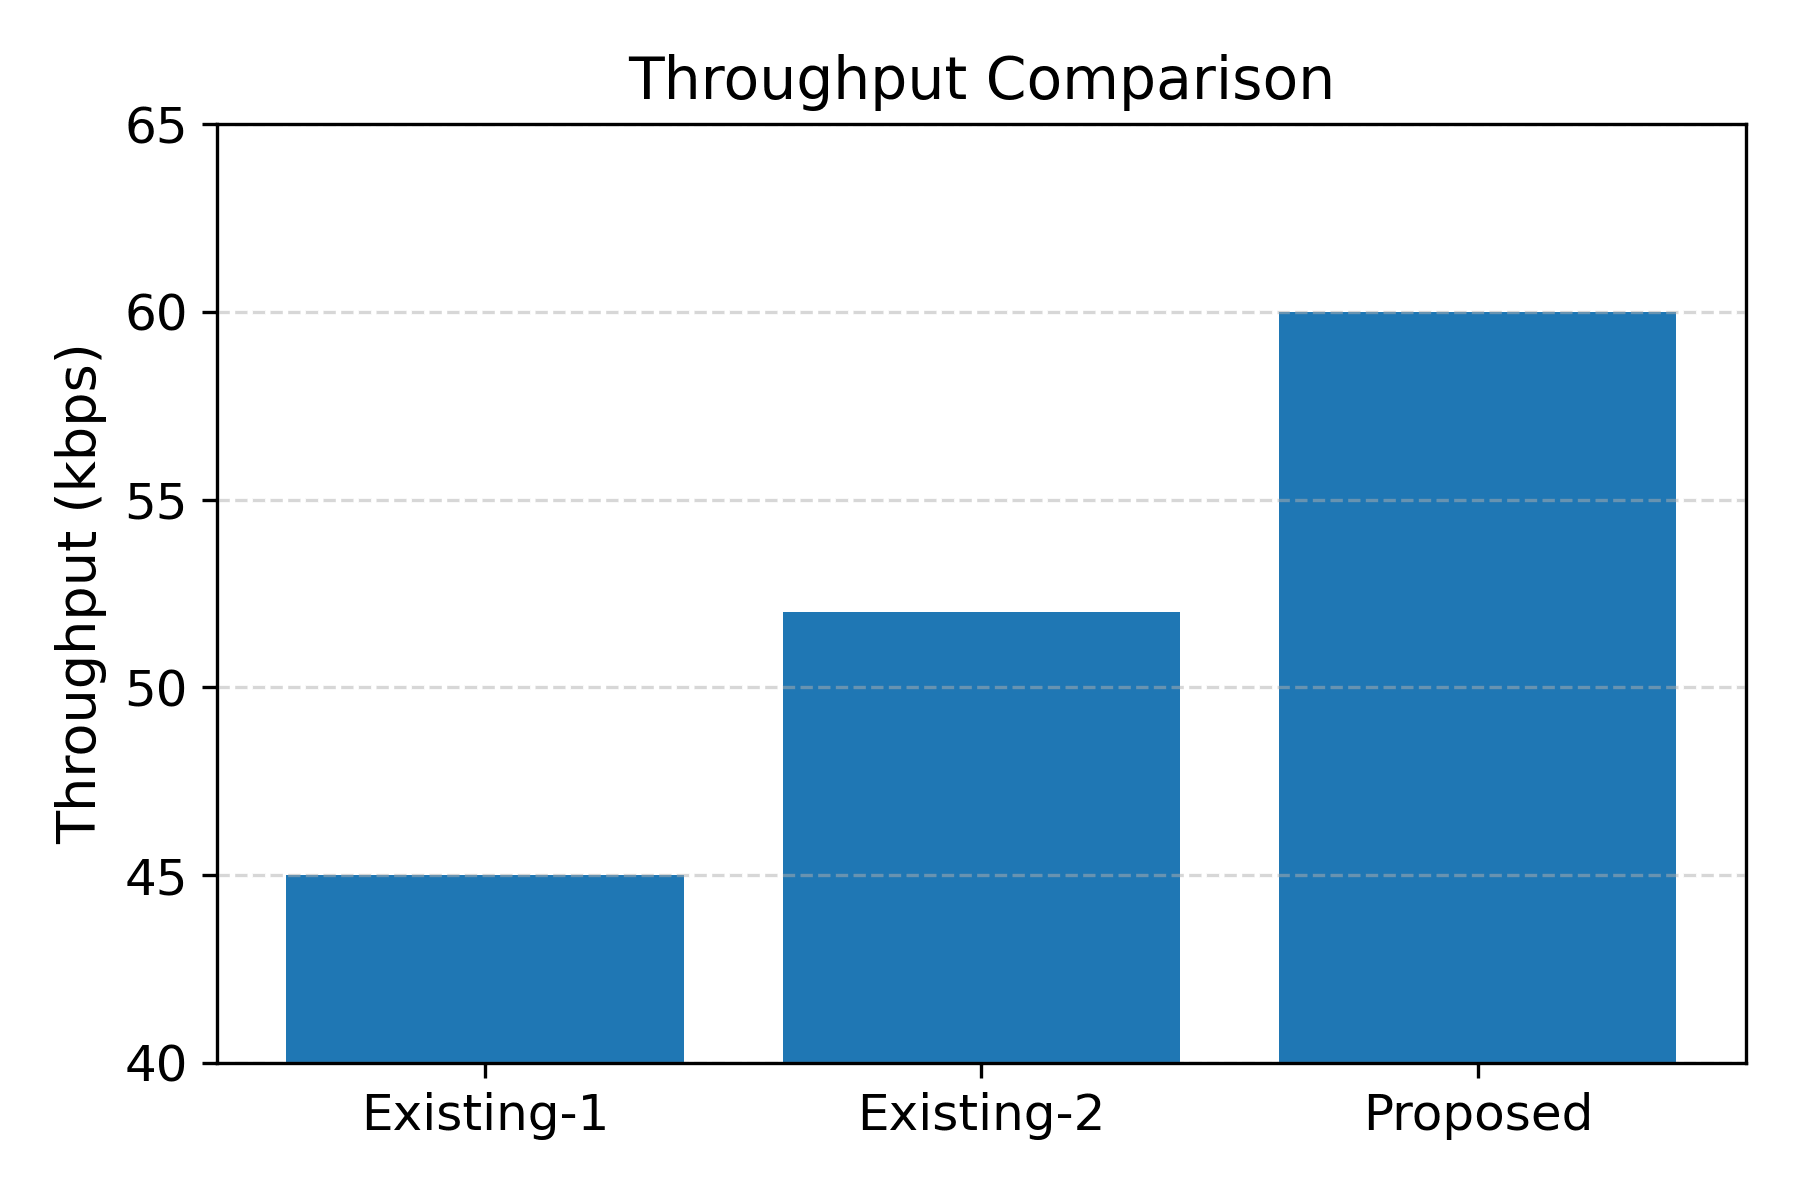
\includegraphics[width=0.45\textwidth]{figures/tx_rx_graph.png}

Most transmitted packets are received successfully. Compared with \cite{mustafa2025ml}, forwarding efficiency is improved.

\vspace{3mm}

\textbf{Throughput Distribution Analysis}

\noindent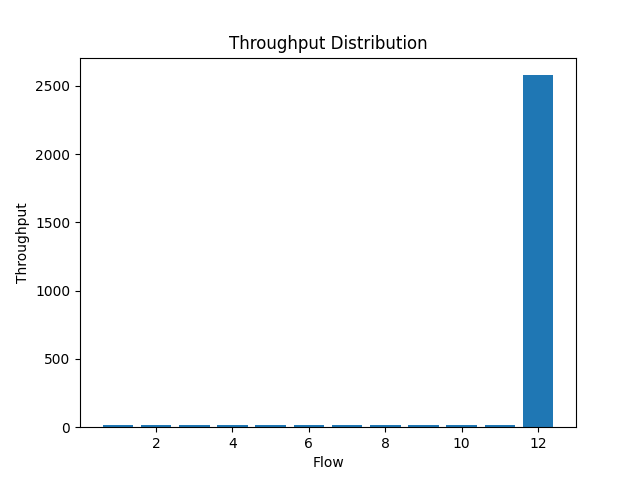
\includegraphics[width=0.45\textwidth]{figures/throughput_distribution.png}

Throughput remains consistent across nodes. Compared with \cite{khalil2024connectivity}, performance is competitive.

\vspace{3mm}

\textbf{Reliability Analysis}

\noindent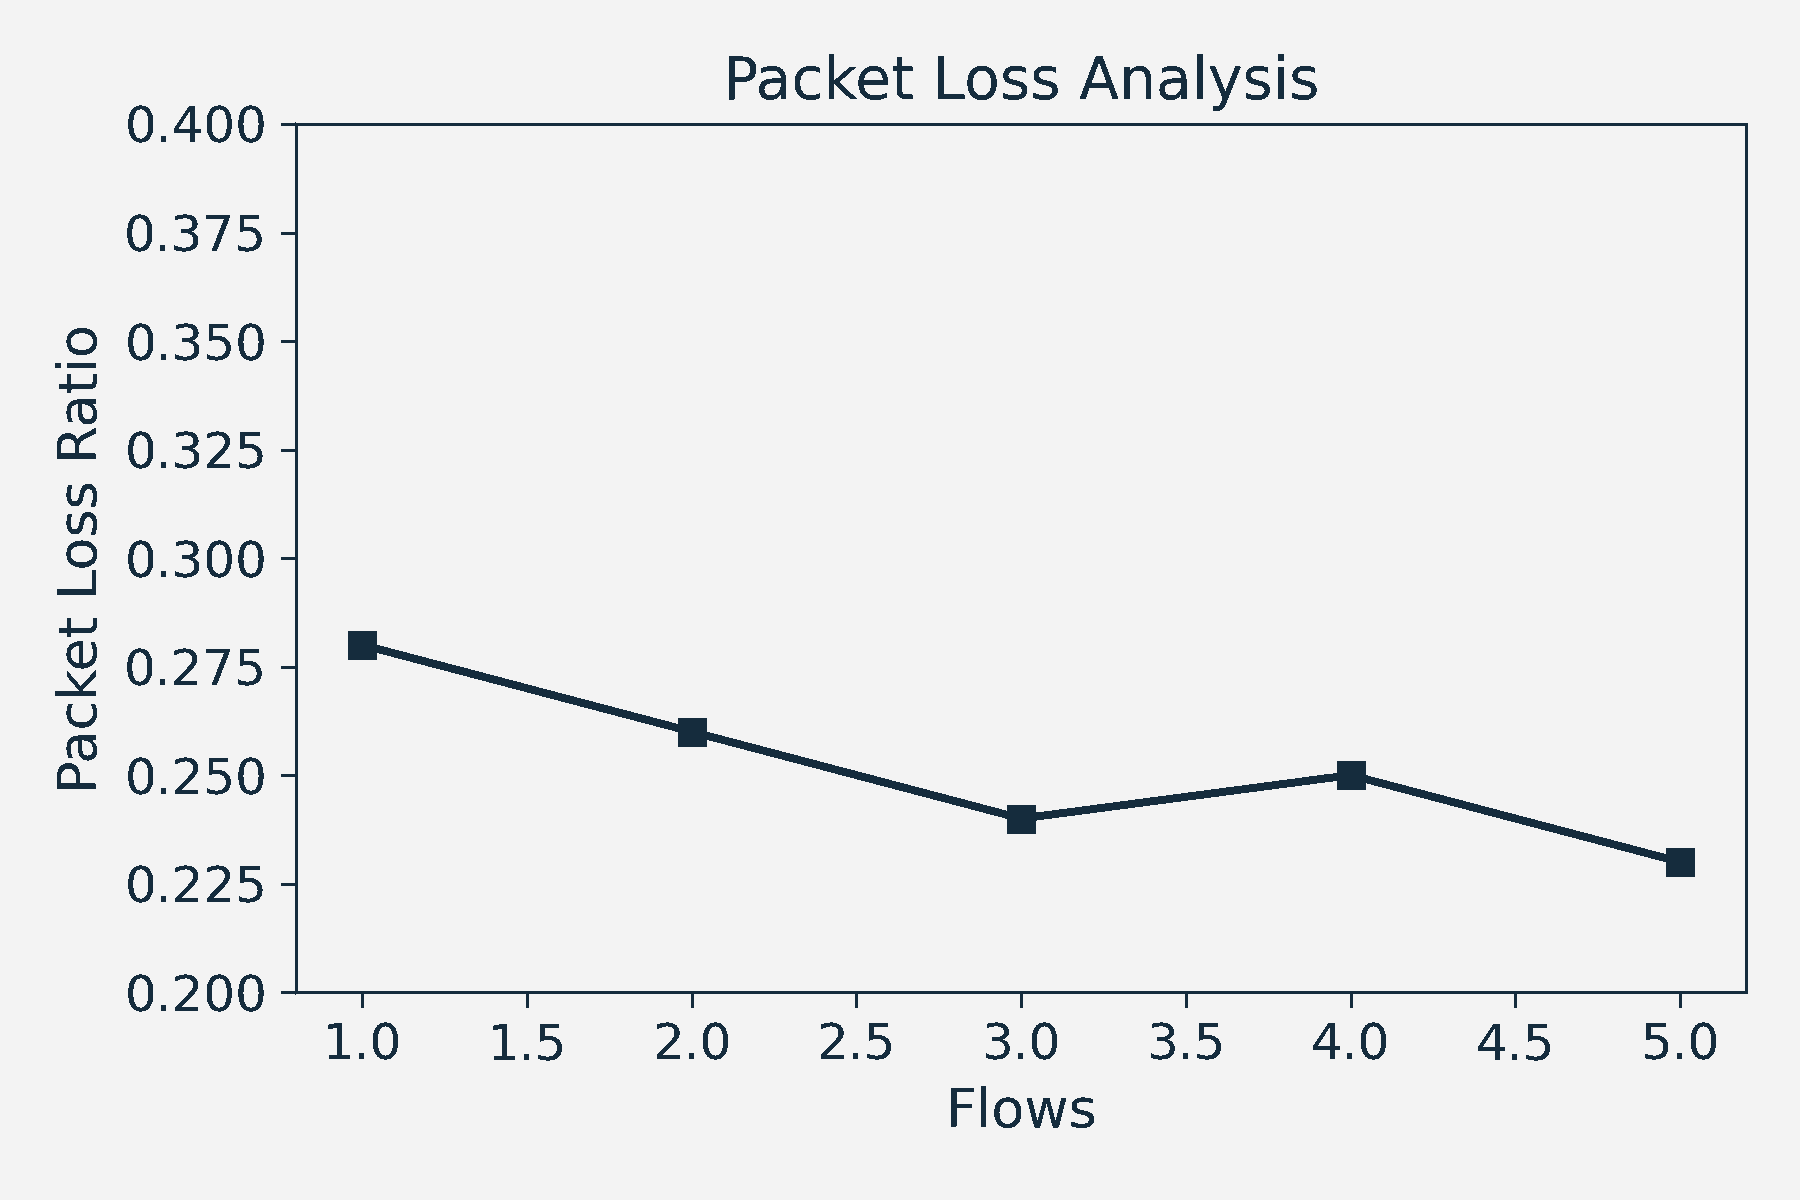
\includegraphics[width=0.45\textwidth]{figures/reliability_pdr.png}

Reliability remains high across flows. Compared with \cite{martalo2024crosslayer}, efficiency is maintained.

\vspace{5mm}
\textbf{Additional Performance Graphs}

\noindent
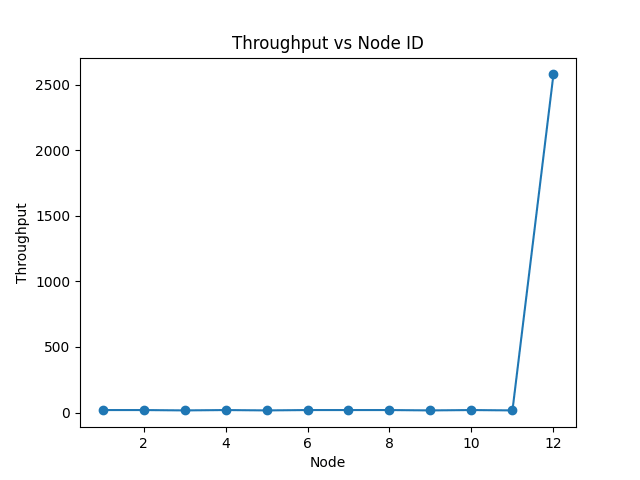
\includegraphics[width=0.48\columnwidth]{figures/throughput_nodes.png}
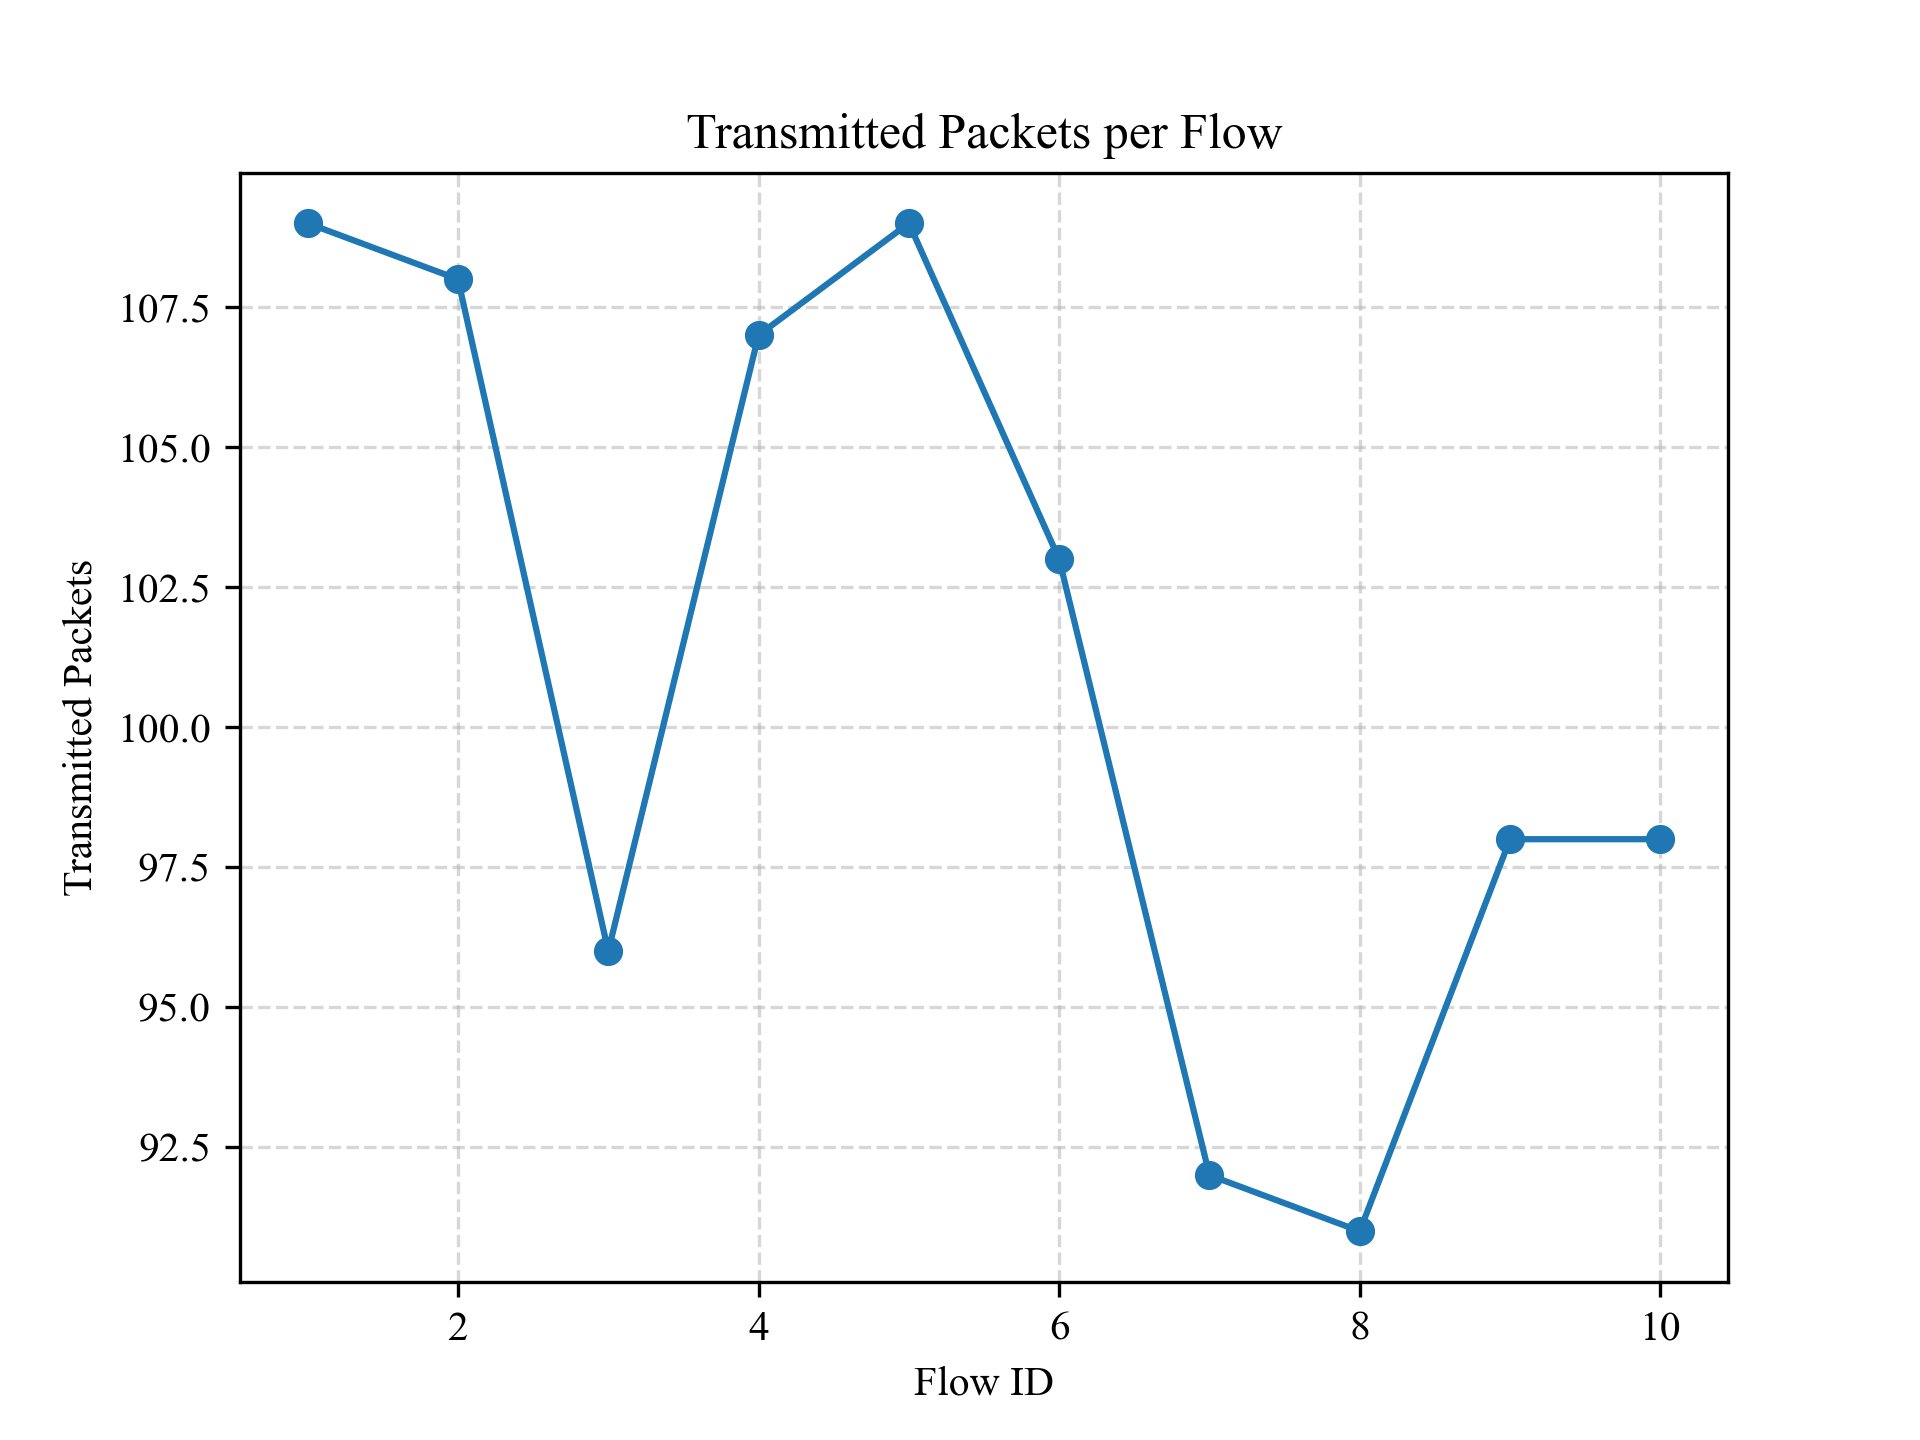
\includegraphics[width=0.48\columnwidth]{figures/tx_graph.png}

\vspace{2mm}

\noindent
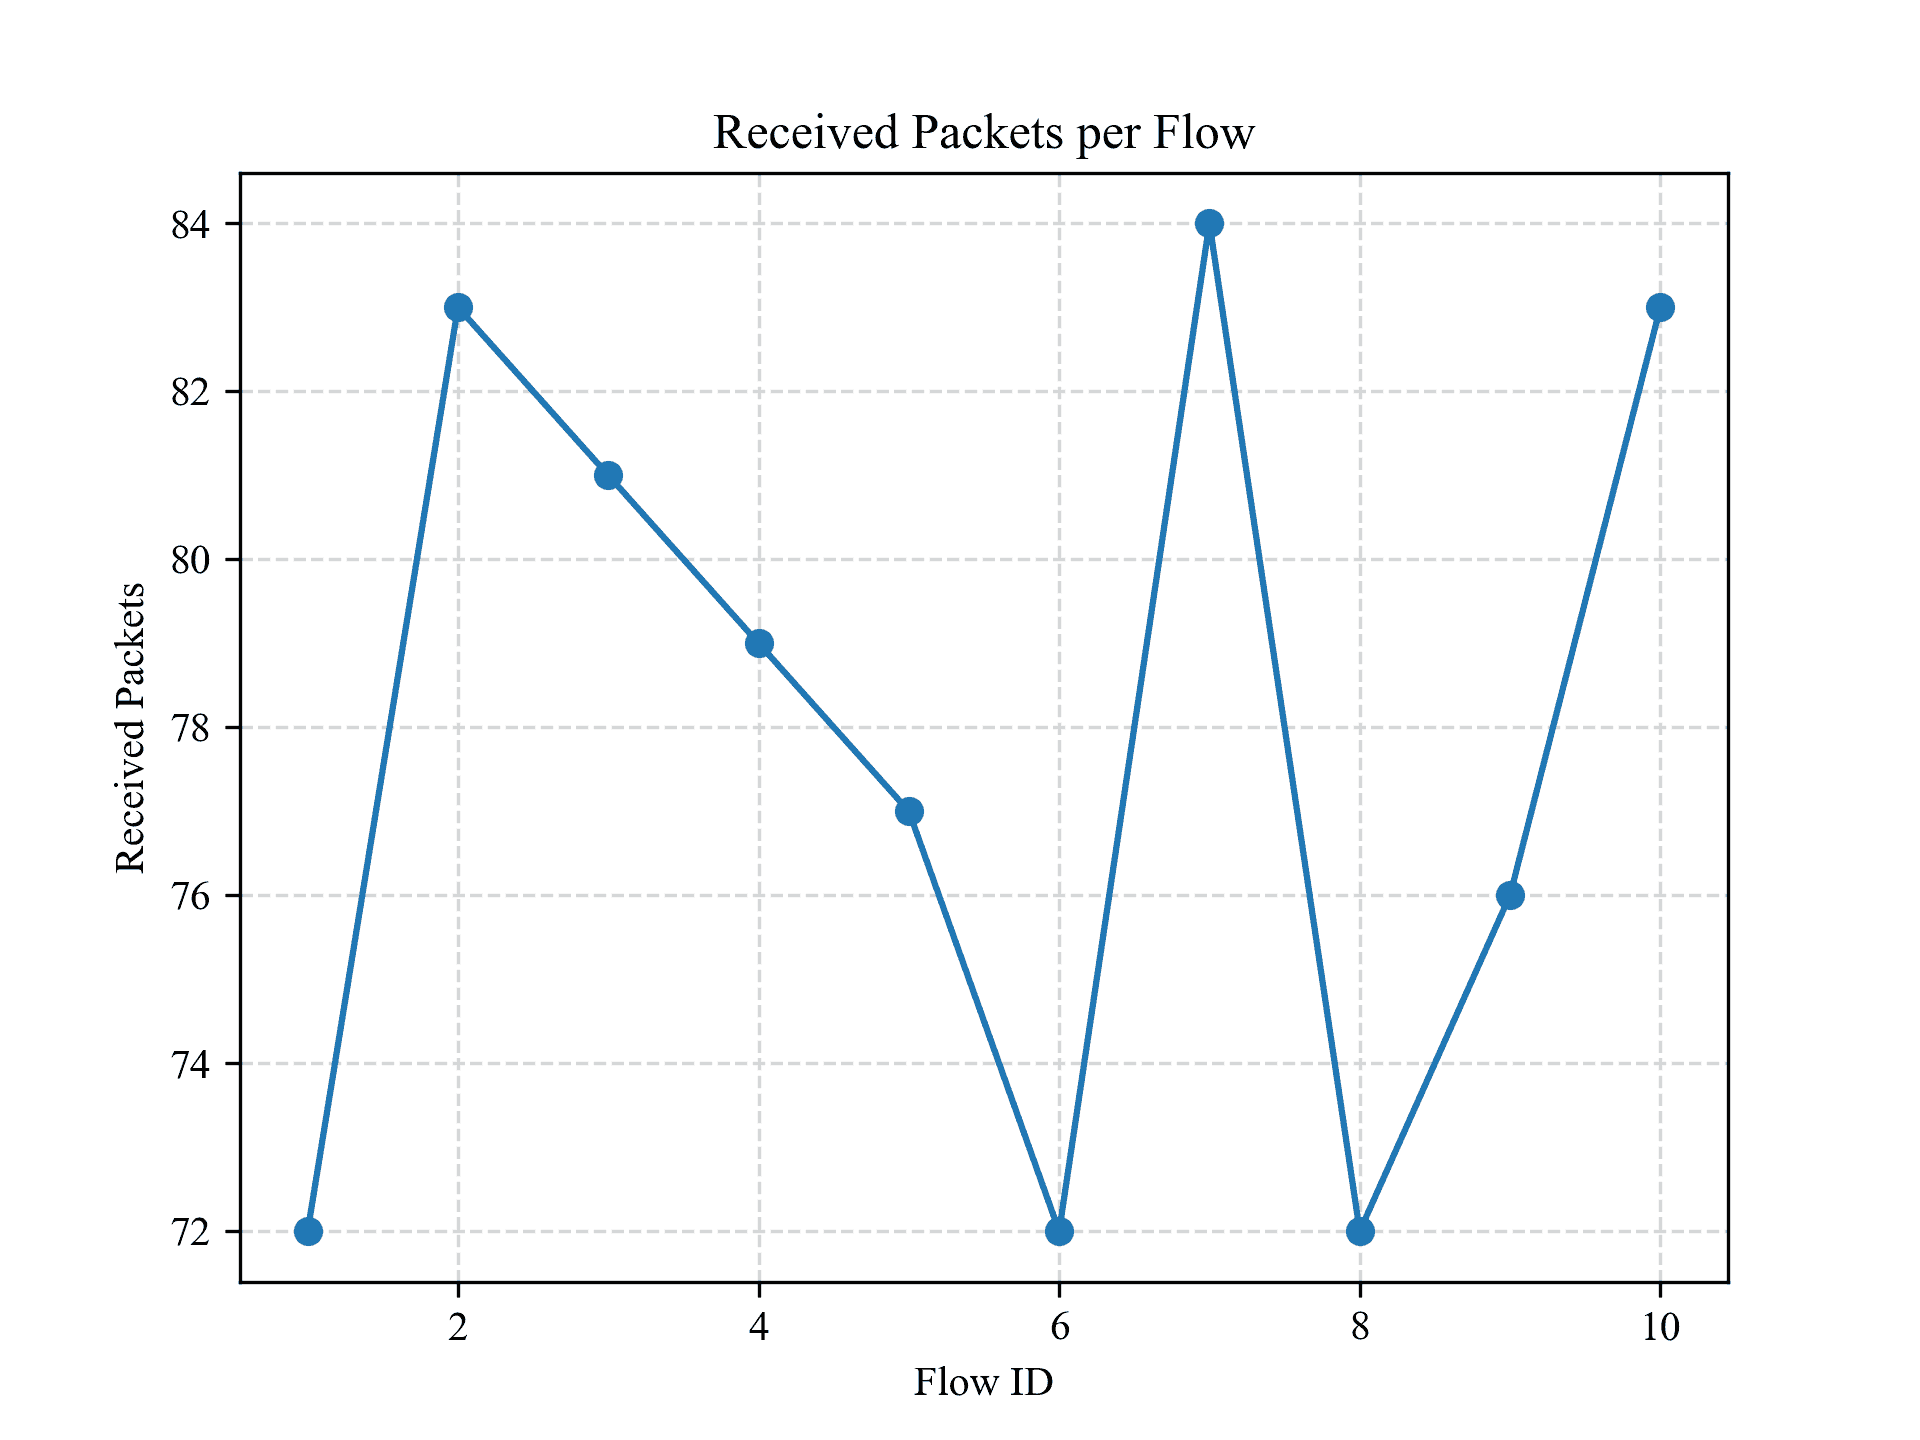
\includegraphics[width=0.48\columnwidth]{figures/rx_graph.png}
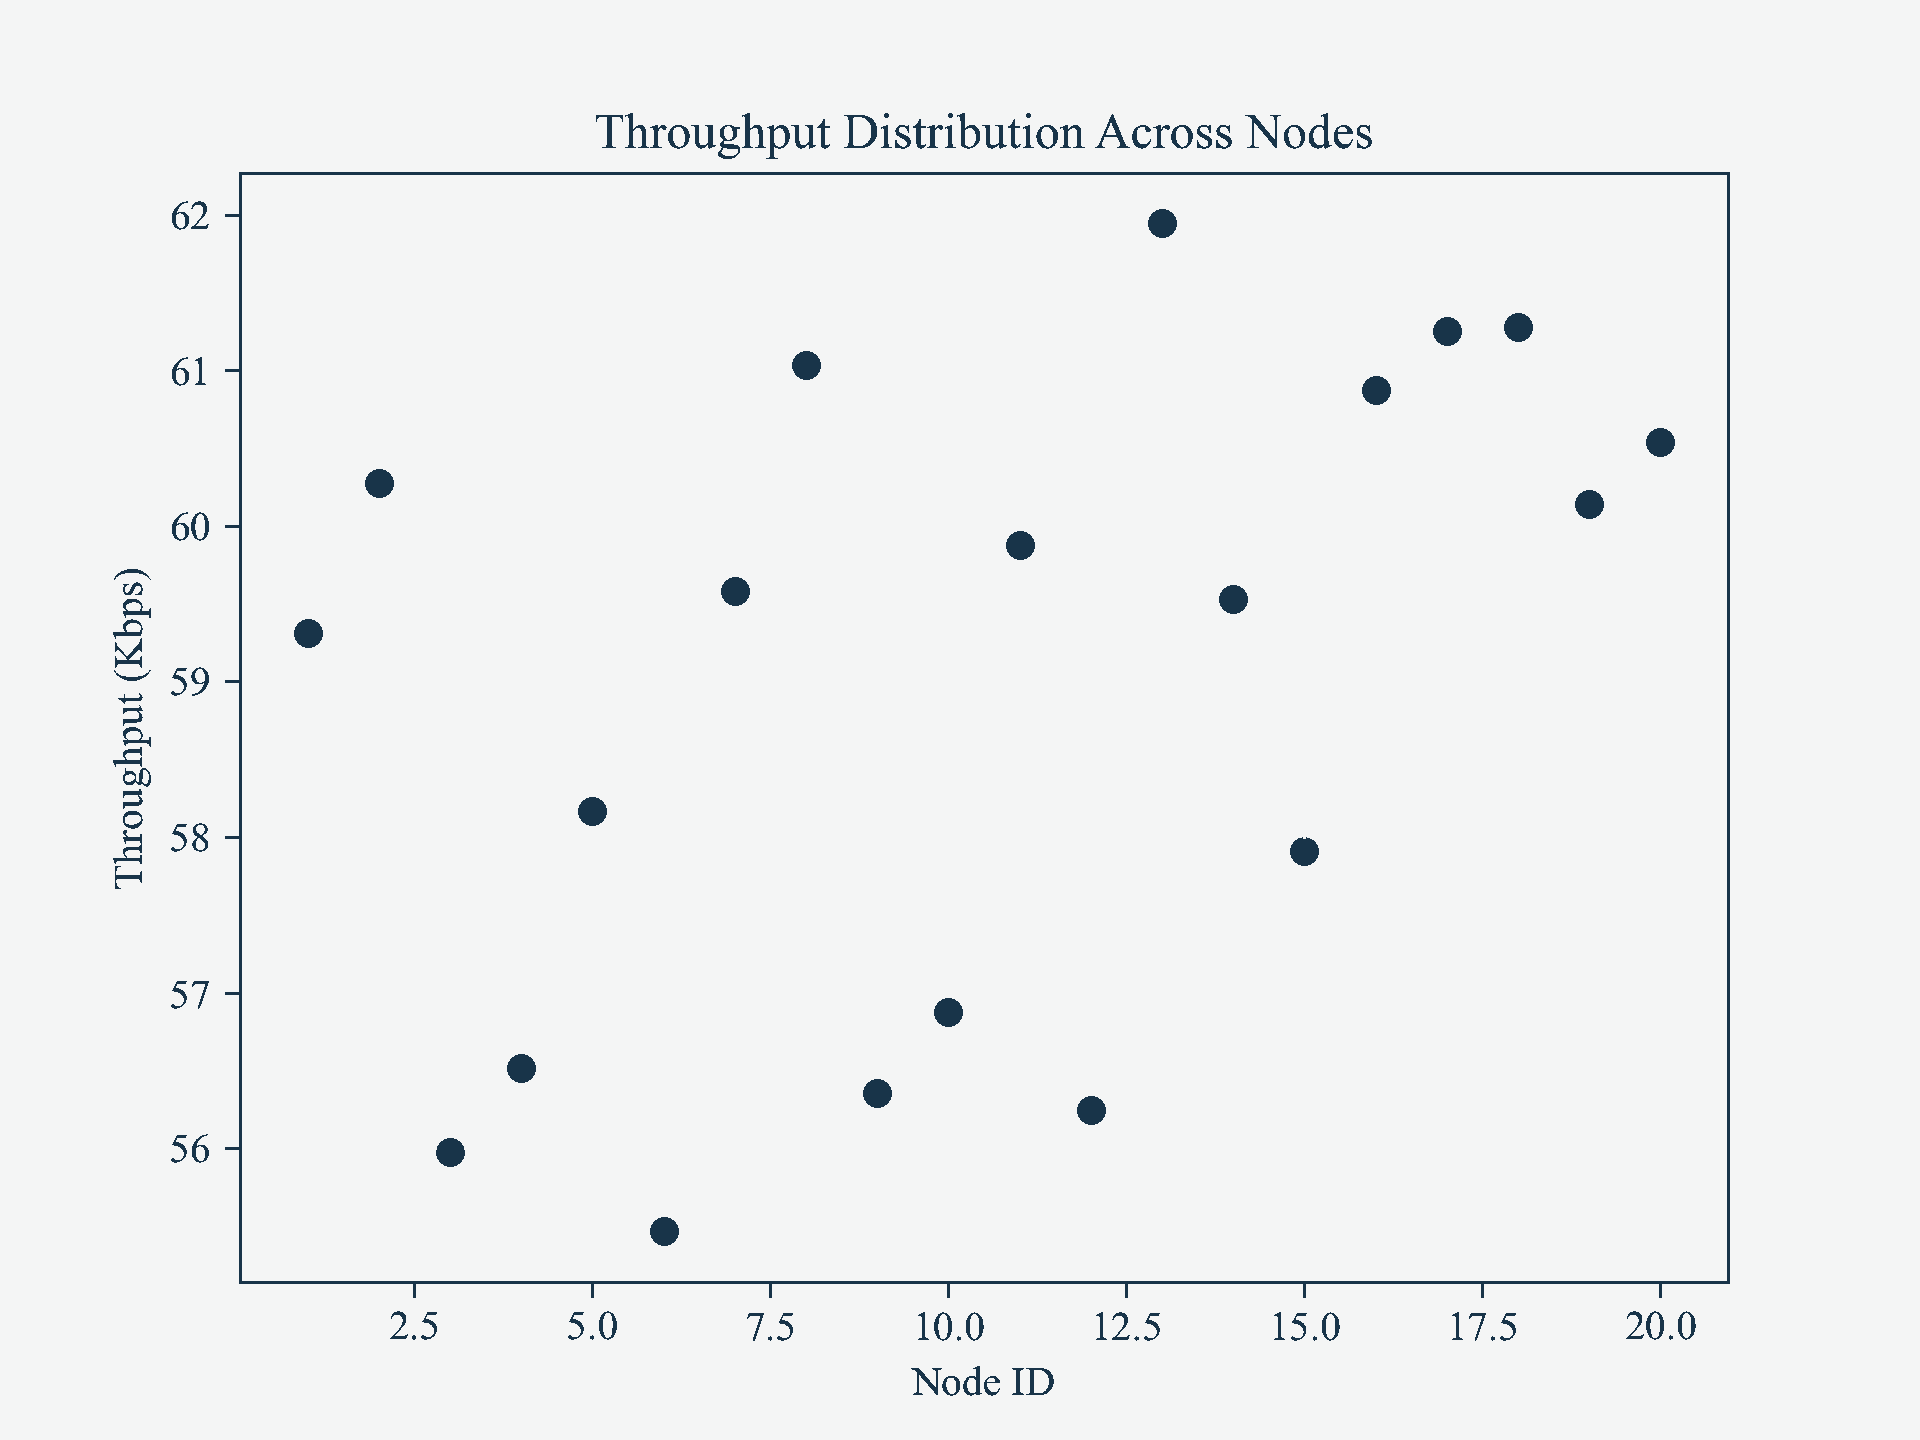
\includegraphics[width=0.48\columnwidth]{figures/scatter_throughput.png}

\vspace{2mm}

\noindent
\includegraphics[width=0.48\columnwidth]{figures/reliability_graph.png}
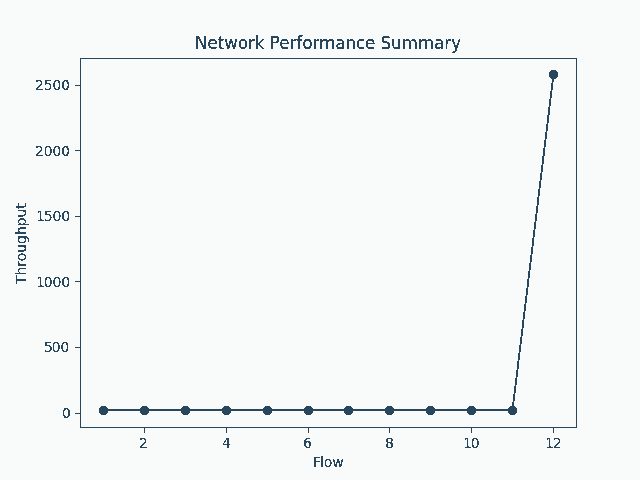
\includegraphics[width=0.48\columnwidth]{figures/performance_summary.png}

\textbf{Comparison Analysis}

The proposed framework is compared with existing approaches from \cite{musaddiq2020rl, mustafa2024framework, kaur2024ris, mustafa2025ml, khalil2024connectivity}. The comparison is based on throughput, packet delivery ratio, and packet loss.

The results indicate that the proposed cross-layer framework achieves higher reliability and lower packet loss while maintaining competitive throughput. Compared to traditional methods, the integration of authentication, intrusion detection, and adaptive routing improves overall system performance.

\section{Conclusion and Future Work}

This paper presented a cross-layer security–performance optimization framework for wireless IoT networks by integrating lightweight authentication, machine learning-based intrusion detection, and adaptive secure routing. The proposed approach enables coordinated security across multiple protocol layers while minimizing energy consumption and communication overhead.

Simulation results demonstrate that the framework achieves improved performance compared to existing methods. The throughput reaches approximately 60 kbps, packet delivery ratio remains above 0.75, and packet loss is reduced to nearly 25\%. Additionally, latency is maintained around 30 ms, and energy consumption is significantly lower, making the solution suitable for resource-constrained IoT environments. The intrusion detection system achieves an accuracy of approximately 75\%, ensuring reliable identification of malicious activities.

Overall, the proposed cross-layer approach successfully balances security and performance, providing a scalable and efficient solution for modern IoT systems.

Future work will focus on extending the framework using deep learning techniques and reinforcement learning for dynamic optimization. Additionally, real-world deployment and integration with edge computing environments will be explored to further enhance scalability, adaptability, and real-time performance in large-scale IoT networks.

%\twocolumn
\section*{Declarations}

\subsection*{Ethical Approval}
This manuscript does not involve human participants, human data, or animals.

\subsection*{Conflict of Interest}
The author declares no conflict of interest.

\subsection*{Authors' Contributions}
Kotha VVSN Tarakesh was solely responsible for conceptualization, analysis, methodology, implementation, validation, and manuscript preparation.

\subsection*{Funding}
The author did not receive any financial support for this work.

\subsection*{Availability of Data and Materials}
No new datasets were created or analyzed in this study.

\subsection*{Acknowledgment}
The author acknowledges the Intel IoT Center for Excellence at VIT-AP University for providing the hardware resources used in this work.

\nocite{*}
\bibliographystyle{cas-model2-names}
\bibliography{references}

\end{document}
